%%%%%%%%%%%%%%%%%%%%%%%%%%%%%%%%%%%%%%%%%%%%%%%%%%%%%%%%%%%%
%%% ELIFE ARTICLE TEMPLATE
%%%%%%%%%%%%%%%%%%%%%%%%%%%%%%%%%%%%%%%%%%%%%%%%%%%%%%%%%%%%
%%% PREAMBLE 
\documentclass[9pt,lineno]{elife}
% Use the onehalfspacing option for 1.5 line spacing
% Use the doublespacing option for 2.0 line spacing
% Please note that these options may affect formatting.
% Additionally, the use of the \newcommand function should be limited.
\newcommand{\beginsupplement}{%
	\setcounter{table}{0}
	\renewcommand{\thetable}{S\arabic{table}}%
	\setcounter{figure}{0}
	\renewcommand{\thefigure}{S\arabic{figure}}%
}

\usepackage{lipsum} % Required to insert dummy text
\usepackage[version=4]{mhchem}
\usepackage{siunitx}
\DeclareSIUnit\Molar{M}

%%%%%%%%%%%%%%%%%%%%%%%%%%%%%%%%%%%%%%%%%%%%%%%%%%%%%%%%%%%%
%%% ARTICLE SETUP
%%%%%%%%%%%%%%%%%%%%%%%%%%%%%%%%%%%%%%%%%%%%%%%%%%%%%%%%%%%%
\title{Regulation of membrane scission in yeast endocytosis}

\author[1]{Deepikaa Menon}
%\author[1,2\authfn{1}\authfn{3}]{Firstname Middlename Familyname}
%\author[2\authfn{1}\authfn{4}]{Firstname Initials Surname}
\author[1*]{Marko Kaksonen}
\affil[1]{Department of Biochemistry, University of Geneva, Geneva, Switzerland}
%\affil[2]{Institution 2}

\corr{Marko.Kaksonen@unige.ch}
%\corr{email2@example.com}{FS}

%\contrib[\authfn{1}]{These authors contributed equally to this work}
%\contrib[\authfn{2}]{These authors also contributed equally to this work}

%\presentadd[\authfn{3}]{Department, Institute, Country}
%\presentadd[\authfn{4}]{Department, Institute, Country}
% \presentadd[\authfn{5}]{eLife Sciences editorial Office, eLife Sciences, Cambridge, United Kingdom}

%%%%%%%%%%%%%%%%%%%%%%%%%%%%%%%%%%%%%%%%%%%%%%%%%%%%%%%%%%%%
%%% ARTICLE START
%%%%%%%%%%%%%%%%%%%%%%%%%%%%%%%%%%%%%%%%%%%%%%%%%%%%%%%%%%%%

\begin{document}

\maketitle

\begin{abstract}

\end{abstract}


\section{Introduction}

Clathrin-mediated endocytosis (CME) is the major endocytic process by which cargo from the cell exterior is incorporated into a Clathrin-coated vesicle that is then transported into the cell interior \citep{Bitsikas2014}. Over 50 different proteins are involved in reshaping a flat plasma membrane into an invagination that eventually forms the vesicle \citep{Kaksonen2018}. Forces that drive the transition from invagination to spherical vesicle in multicellular eukaryotes are provided by the GTPase Dynamin \citep{Grigliatti1973, Sweitzer1998, Ferguson2007,Takei1995, Galli2017}. Dynamin is now known to interact via its proline-rich-domain with SH3 domains of crescent-shaped N-BAR proteins like Endophilin and Amphiphysin  \citep{Grabs1997,Cestra1999,Farsad2001,Ferguson2009,Meinecke2013b}. Conformation changes of Dynamin recruited to N-BAR molecules cause constriction of the underlying invaginated membrane, resulting in vesicle formation  \citep{Shupliakov1997,Zhang2001,Zhao2016}.

~\\

In yeast, CME is the only pathway for uptake of cargo, and involves a similar membrane transformation as in other eukaryotes. Most mammalian CME proteins have homologues in yeast: these proteins drive the establishment of endocytic sites, form the mechanical link between membrane and actin proteins \citep{Kaksonen2018}. Actin nucleation and polymerization drives the formation of tubular invaginations in yeast \citep{Kubler1993a, Kaksonen2003}. The role of Dynamin in this process has been debated:  yeast dynamin-like protein Vps1 has a major role in the Golgi and other membrane trafficking pathways \citep{Rothman1990,Peters2004,Hoepfner2001}, and been proposed to interact with endocytic proteins \citep{Nannapaneni2010b, Yu2004,Smaczynska-deRooij2012}. Its contribution to CME is however, still debated \citep{GoudGadila2017,Kishimoto2011}. In yeast cells, what causes membrane scission is thus unclear, although the yeast N-BAR Rvs complex (a heterodimeric complex of the proteins Rvs161 and Rvs167) has been identified as an important component of the scission module \citep{Munn1995,Kaksonen2005,DHondt2000,Kishimoto2011}. The two Rvs proteins are homologues of N-BAR proteins Amphiphysin and Endophilin \citep{Friesen2006,Youn2010}. Deletion of Rvs167 reduces scission efficiency by nearly 30\% and reduces the invagination lengths at which scission occurs \citep{Kaksonen2005,Kukulski2012}. Apart from the canonical N-BAR domain which forms the crescent-shaped structure,  Rvs167 has a Glycine-Proline-Alanine rich (GPA) region and a C-terminal SH3 domain \citep{Sivadon1997}. The GPA region is thought to act as a linker with no other known function, while loss of the SH3 domain affects budding pattern and actin morphology \citep{Sivadon1997}. Most Rvs deletion phenotypes can be rescued by expression of the BAR domains alone \citep{Sivadon1997}, suggesting that the BAR domains are the functional unit of the Rvs complex.

The Rvs complex can tubulate liposomes in vitro, indicating that the BAR domains can impose curvature on membranes \citep{Youn2010}. However, Rvs arrives at endocytic sites when membrane tubes are already formed: curvature sensing rather than generation is the likely interaction of the complex with endocytic sites \citep{Kukulski2012,Picco2015}. Rvs molecules arrive at endocytic sites about 4 seconds before scission, and disassemble rapidly at the time of scission \citep{Picco2015}, consistent with a role in scission. While it is shown to be involved in the last stages of endocytosis, a mechanistic understanding of the influence of Rvs on scission remains incomplete. 

~\\
Several scission models have been proposed that allow a major role for Rvs and are tested in this work. Although the yeast Dynamin Vps1 lacks a canonical BAR-protein binding site \citep{Bui2012,Moustaq2016}, it may be recruited via a different mechanism and induce scission. Liu et al., proposed that Synaptojanins may selectively hydrolyze lipids at endocytic sites, causing line tension between two lipid types that results in scission \citep{Liu2009}. Protein friction along the membrane invagination has been proposed as a mechanism by which scission may occur \citep{Simunovic2017b}. We used quantitative live-cell imaging and genetic manipulation in Saccharomyces cerevisiae to test these theories and investigate the function of Rvs in endocytosis. We found that Rvs is recruited to endocytic sites by both BAR and SH3 domains. Of several potential actin-interacting binding partners of the SH3 domains such as Myo3, Myo5, Vrp1, Abp1 \citep{Lila1997,Colwill1999,Madania1999,Liu2009}. we found that type I myosin Myo3 interacts with Rvs SH3 domains. Our data also suggests that the aforementioned theories of membrane scission are unlikely to sever the membrane in yeast, and that actin polymerization likely generates the forces required for scission. 

%INTRO?
%In mammalian cells, disruption of Synaptojanin genes results in cellular accumulation of PIP2 at endocytic sites. Coated vesicles gather at the plasma membrane, suggesting a role for lipid hydrolysis in releasing coat proteins from nascent vesicles (ref?). As an alternate to forces from Dynamin constriction, Liu et al (refliu) have proposed that an interaction between PiP2-hyrdolyzing Synaptojanins and BAR proteins could drive membrane scission. In this model Rvs BAR domains would form a scaffold on the membrane tube, preventing hydrolysis of underlying PIP2. Synaptojanin would arrive at inavaginated membranes, and hydrolyse unprotected PIP2. This generates a lipid boundary between BAR-protected PIP2 at the tube and hydrolyzed PIP2 at the bud tip. A line tension thus formed at the interphase between the two lipid types would then generate enough force to pinch off a vesicle.


\section{Results}

\subsection{Rvs167, rather than Vps1 influences coat movement}

Yeast Dynamin-like protein Vps1 does not contain a Proline Rich Domain, which in mammalian cells is required for recruitment to endocytic sites \citep{Grabs1997,Cestra1999,Farsad2001,Meinecke2013b}. In spite of the lack of a stereotypical interaction domain, some works have reported its recruitment to endocytic proteins, including to N-BAR protein Rvs167 \citep{Yu2004,Nannapaneni2010b,Rooij2010}. The question of whether or not Vps1 has a function at endocytic sites has been obfuscated by potential tagging-induced dysfunction of Vps1 molecules. Vps1 tagged both N- and C-terminally with GFP constructs failed to co-localize with endocytic protein Abp1 in our hands, consistent with other work that observed localization only with other parts of the trafficking pathway \citep{GoudGadila2017}. We argued that even if tagging Vps1 induced defects in its localization and/or function, its contribution to endocytosis could be examined by observing the dynamics of other endocytic proteins in cells lacking Vps1. The canonical interaction partner of Vps1- Rvs167- localizes to endocytic sites, and has a role in scission, although it is unclear what that is \citep{Kukulski2012,Picco2015}. In order to determine the roles of these proteins in endocytic scission, we studied cells lacking Vps1 and Rvs167, and compared against wild-type (WT) cells (Fig.\ref{vps}A-F).

~\\
Vps1 deletion was confirmed by sequencing the gene locus, and these cells showed a previously reported \citep{Rothman1986}  growth phenotype at high temperatures (Fig.\ref{vps_growthassay}). Scission efficiency was quantified by tracking the endocytic coat protein Sla1 tagged at the C-terminus with eGFP (Fig.\ref{vps}C). Upon actin polymerization, the endocytic coat moves into the cytoplasm along with the membrane as it invaginates \citep{Skruzny2012}. Movement of coat protein Sla1 thus acts as a proxy for the growth of the plasma membrane invagination. Membrane retraction, that is, inward movement and subsequent retraction of the invaginated membrane back towards the cell wall is a scission-specific phenotype \citep{Kaksonen2005}. Retraction rates do not significantly increase in  \textit{vps1$\Delta$} cells compared to the WT (Fig.\ref{vps}C).


\begin{figure}[h]
	\centering
	\includegraphics
	[width=0.8\hsize]{/Users/deepikaa/Desktop/scission_paper/figures/fig1/final/vpsdel_27.pdf}
	\caption{\textbf { \textit{vps1$\Delta$} and \textit{rvs167$\Delta$} deletion} 
		\textbf{A:} Sinlge slices from time lapse movies of WT,  \textit{vps1$\Delta$}, and  \textit{rvs167$\Delta$} cells expressing Sla1-eGFP. Scale bar= 2{\textmu}m. \textbf {B:} Representative kymographs of Sla1-eGFP and Rvs167-eGFP patches in WT,  \textit{vps1$\Delta$}, and  \textit{rvs167$\Delta$} cells from time lapse movies. Scale bar for Sla1-egfp = 20(s), scale bar for Rvs167-eGFP = 5(s). \textbf {C:} Scission efficiency in WT,  \textit{vps1$\Delta$}, and  \textit{rvs167$\Delta$} cells. Error bars are standard deviation, p values from t-test, *= p $\leq$0.05, **= p$\leq$0.01, ***=p$\leq$0.001. \textbf {D:} Averaged centroid positions of Sla1-eGFP in WT and  \textit{vps1$\Delta$}  cells. \textbf {E:}  Averaged position of Rvs167-eGFP in WT and  \textit{vps1$\Delta$}  cells.\textbf {F:} Averaged position of Sla1-eGFP in WT, and successful and retracted Sla1-eGFP positions in \textit{rvs167$\Delta$} cells. All averaged positions were aligned in x axis to begin inward movement at time=0(s), and aligned in the y axis to a starting position = 0(nm). } 
	\label{vps}
\end{figure}


~\\
The total movement of the endocytic coat (Fig.\ref{vps}D,E) gives an indication of when invagination has undergone scission: greater movement would imply defects in the scission mechanism. In order to study this  movement , the averaged centroid trajectory of ~50 Sla1-eGFP patches in \textit{vps1$\Delta$} and WT cells were tracked and compared (Fig.\ref{vps}D). In brief: yeast cells expressing fluorescently-tagged endocytic proteins were imaged at the equatorial plane. Since membrane invagination progresses perpendicularly to the plane of the plasma membrane, proteins that move into the cytoplasm during invagination do so in the imaging plane. Centroids of Sla1 patches- each patch being an endocytic site- were tracked in time and averaged. This provided an average centroid that could be followed with high spatial and temporal precision \citep{Picco2015}. Averaged centroid movement of Sla1-eGFP in WT cells was linear to about 140nm (Fig.\ref{vps}D). Sla1 movement in \textit{vps1$\Delta$} cells had the same magnitude of movement (Fig.\ref{vps}D). In spite of slight differences in the rates of movement, the total movement- and so the depth of endocytic invagination- did not change.
%When different endocytic proteins are simultaneously imaged with Actin Binding Protein Abp1, Abp1 provides a frame of reference to which all the other proteins can be aligned. Abp1 is used because it is abundant at endocytic sites and therefore easily imaged. Time=0 is established as the peak of the Abp1 fluorescence intensity in respective co-tagged strains strains. Abp1 fluorescent intensity maxima in wild-type cells is concomitant with the peak of Rvs167 fluorescent intensity and is time window in which scission occurs (ref2andrea, refwanda).  

~\\
Centroid tracking has shown that the number of molecules of Rvs167 peaks at the time of  scission, and is followed by a rapid loss of fluorescent intensity, simultaneous with a sharp jump of the centroid into the cytoplasm \citep{Picco2015}. This jump, also seen in Rvs167-GFP kymographs (Fig.\ref{vps}B), is interpreted as loss of protein on the membrane tube, causing an apparent spatial jump to the protein localized at the base of the newly formed vesicle. Kymographs of Rvs167-GFP (Fig.1B), as well as Rvs167 centroid tracking (Fig.\ref{vps}E) in Vps1 deleted cells showed the same jump as in WT. 

~\\
The Rvs complex is composed of Rvs161 and Rvs167 dimers (Boeke et al. 2014) so deletion of Rvs167 effectively removes both proteins from endocytic sites. We quantified the effect of \textit{rvs167$\Delta$}  on membrane invagination (Fig.\ref{vps}A-C,F). Only 73\% of Sla1 patches undergo successful scission in \textit{rvs167$\Delta$}  cells (Fig.\ref{vps}C). Similar scission rates have been measured in other experiments \citep{Kaksonen2005}, and suggest failed scission in the remaining 27\% of endocytic events. Coat movement both of retractions and of successful endocytic events were quantified (Fig.1F) as described earlier. Sla1 centroid movement in both successful and retracting endocytic events in \textit{rvs167$\Delta$}  cells look similar to WT up to about 50nm (Fig.\ref{vps}F). In WT cells, Abp1 intensity begins to drop at scission time (Fig.\ref{wt_alignment}); similarly, in successful endocytic events, Abp1 intensity drops after Sla1 centroid has moved about 100nm suggesting that scission occurs at invagination lengths between 60 -100 nm (Fig.\ref{rvsdel_alignment}). That membrane scission occurs at shorter invagination lengths than in WT is corroborated  by the smaller vesicles formed in \textit{rvs167$\Delta$}  cells by Correlative light and electron microscopy (CLEM) \citep{Kukulski2012}. CLEM has moreover shown that Rvs167 localizes to endocytic sites after the invaginations are about 60nm long \citep{Kukulski2012}. Sla1 movement in \textit{rvs167$\Delta$} indicates therefore that membrane invagination is unaffected till Rvs is supposed to arrive. 


%DISCUSSION?
%This indicates that first, membrane scission can occur at invagination lengths of 80nm. Then, that the arrival of Rvs prevents membrane scission at 80nm and allows further membrane invagination. In retraction events, after inward movement, the Sla1 centroid moves back towards the starting position, that is, to the plasma membrane. 



\subsection{Synaptojanins likely influence vesicle uncoating, but not scission dynamics.}

As Vps1 did not appear to influence membrane scission, we proceeded to test another scission model. The lipid hydrolysis model proposes that deletion of yeast synaptojanins would inhibit scission and therefore result in longer invaginations \citep{Liu2009}.  Three Synaptojanin-like proteins have been identified in S. cerevisiae: Inp51, Inp52, and Inp53. Inp51-eGFP exhibits a diffuse cytoplasmic signal, Inp52-eGFP localizes to cortical patches that are endocytic sites (Fig.\ref{inp}A, supplement) and Inp53 localizes to patches within the cytoplasm (Fig.\ref{inp}A, \citep{Bensen2000}). Since Inp52 localizes to endocytic sites, we began with determining the spatial and temporal recruitment of Inp52 within the endocytic machinery. We aligned the averaged centroid of Inp52 in space and time to other endocytic proteins \citep{Picco2015}. In order to do this, we imaged Inp52-eGFP simultaneously with Abp1-mCherry, and did the same with Sla1-eGFP and Rvs167-eGFP. Using Abp1 as the common reference frame, we were able to compare the arrival of the different proteins with respect to that of Abp1. We assigned as time =0 (s) the fluorescent intensity maximum of Abp1, which in WT cells is concomitant with membrane scission, and also coincides with the maximum of the Rvs167 fluorescent intensity (Fig.\ref{vps}A, \ref{vpsdel_alignment}). On the y axis, 0 (nm) indicates the position of the Sla1 centroid; positions of the other centroids are in relation to the Sla1 centroid. Inp52 molecules arrived in the late stage of endocytosis after Rvs167 arrival, and localized to the invagination tip, suggesting a potential role in membrane scission (Fig.\ref{inp}B).


\begin{figure}
	\centering
	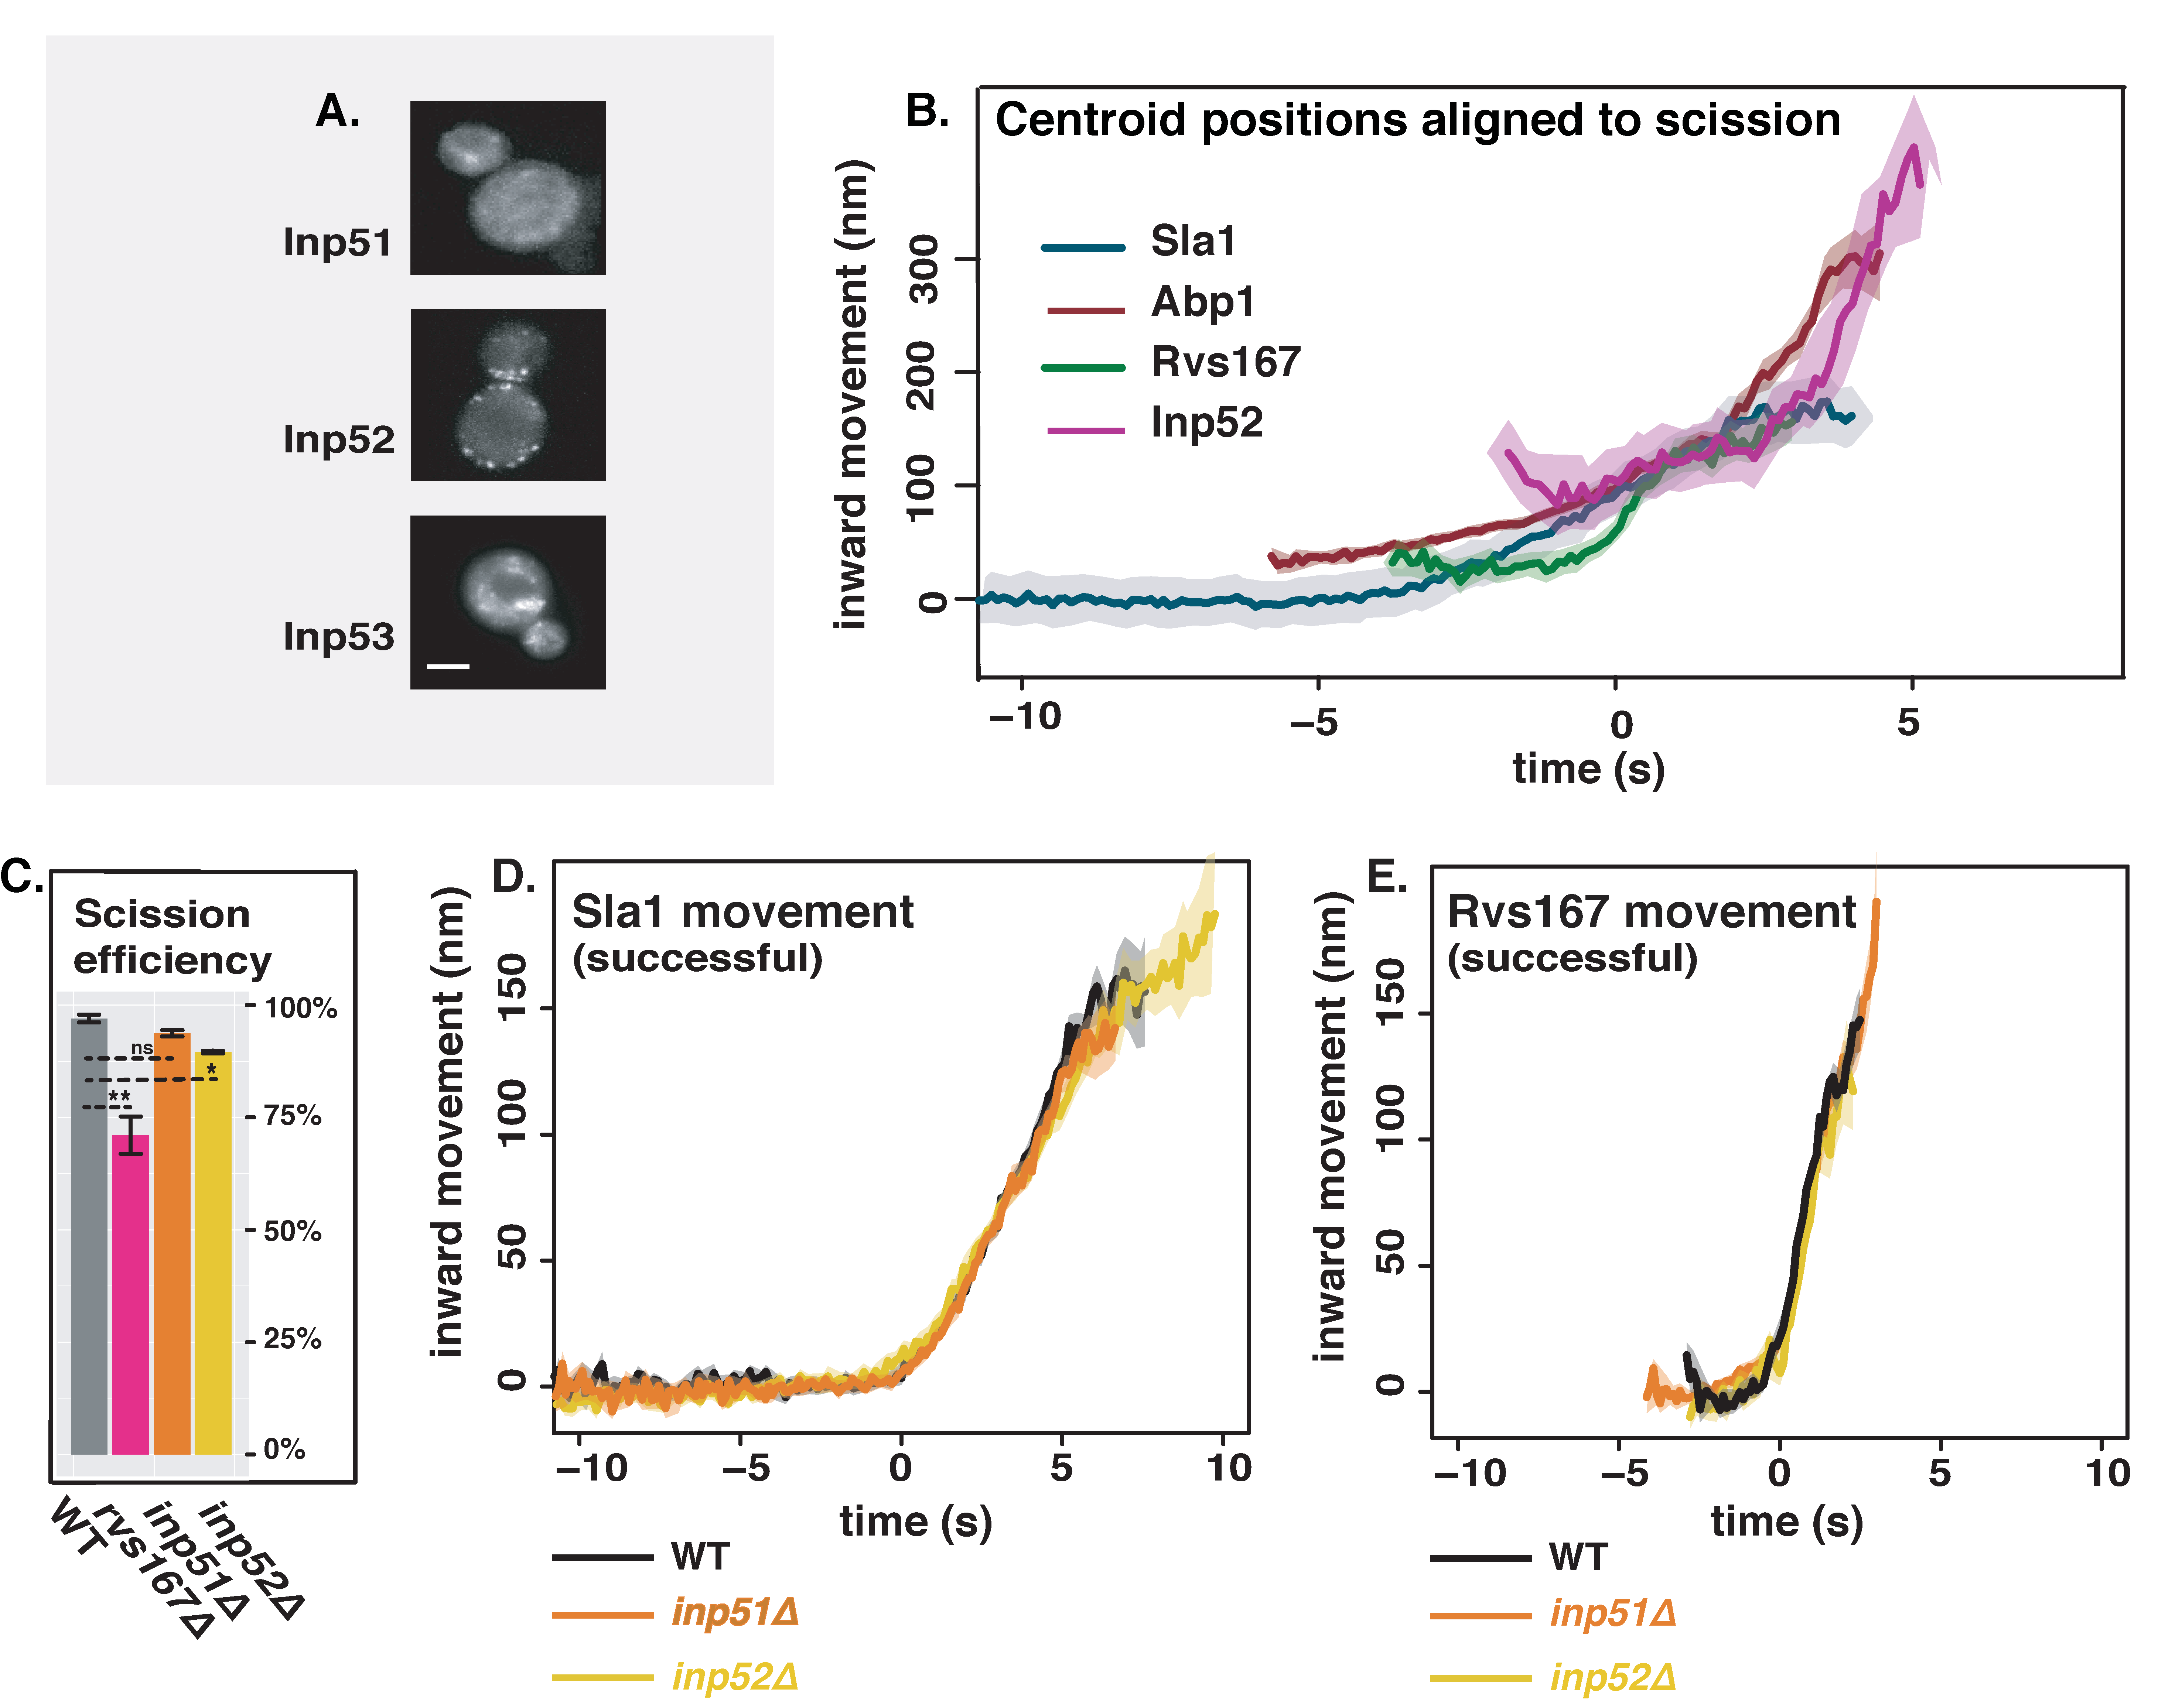
\includegraphics
	[width=0.8\hsize]{/Users/deepikaa/Desktop/scission_paper/figures/fig2/inp8.pdf}
	\caption{\textbf { Involvement of yeast Synaptojanin-like proteins in endocytosis } 
		\textbf{A:} Cells endogenously tagged with Inp51-, Inp52-, and Inp53-eGFP. \textbf{B:} Inp52 centroid trajectory was aligned in space and time to other endocytic proteins. \textbf{C:} Sla1 retraction rates in \textit{inp51$\Delta$} and  \textit{inp52$\Delta$} cells compared to WT and  \textit{rvs167$\Delta$}. Error bars are standard deviation, with p values from t-test, *= p$\leq$0.05, **= p$\leq$0.01, ***=p$\leq$0.001. \textbf{D:} Averaged centroid positions of Sla1-eGFP in WT, \textit{inp51$\Delta$}, and \textit{inp52$\Delta$}  cells. \textbf{E:} Averaged centroid positions of Rvs167-eGFP in WT, \textit{inp51$\Delta$}, and \textit{inp52$\Delta$}  cells.}
	\label{inp}
\end{figure}

Inp53 was not investigated further, as its localization conformed with other literature that found that it is involved in the golgi trafficking pathway and not endocytosis \citep{Bensen2000}. Although we were unable to observe localization of Inp51 at endocytic sites, deletion of Inp51 has been shown to exacerbate the effect of \textit{inp52$\Delta$} on membrane retraction \citep{Liu2009}, so both Inp51 and Inp52 were tested as potential scission regulators.

~\\

Dynamics of Sla1-eGFP and Rvs167-eGFP in \textit{inp51$\Delta$} and \textit{inp52$\Delta$} cells were compared against the WT  (Fig.\ref{inp}C-E). Scission efficiency did not significantly decrease in \textit{inp51$\Delta$} compared to the WT, but showed a slight decrease in \textit{inp52$\Delta$} cells (Fig2C). Total movement of Sla1 and Rvs167 centroids in \textit{inp51$\Delta$} were the same as in WT  (Fig.\ref{inp} D,E), while Rvs167 assembly and disassembly took longer (Fig.\ref{inpdel_supplement}).   Rvs167 centroid, after the inward movement, appeared to persist compared to the WT, likely because of a delay in Rvs167 disassembly from the newly formed vesicle. In \textit{inp52$\Delta$} cells, Sla1 movement had the same magnitude and rate as in WT, but Sla1-eGFP signal is persistent after inward movement scission (Fig.\ref{inp}D). Rvs167 and Sla1 disassembly were delayed in \textit{inp52$\Delta$} cells compared to WT (Fig.\ref{inp}supplement1). This data are consistent with Synaptojanin involvement in assembly and disassembly of coat and scission proteins at endocytic sites rather than in membrane scission. 






\subsection{Rvs BAR domains recognize membrane curvature in-vivo}

\begin{figure}[h]
	\centering
	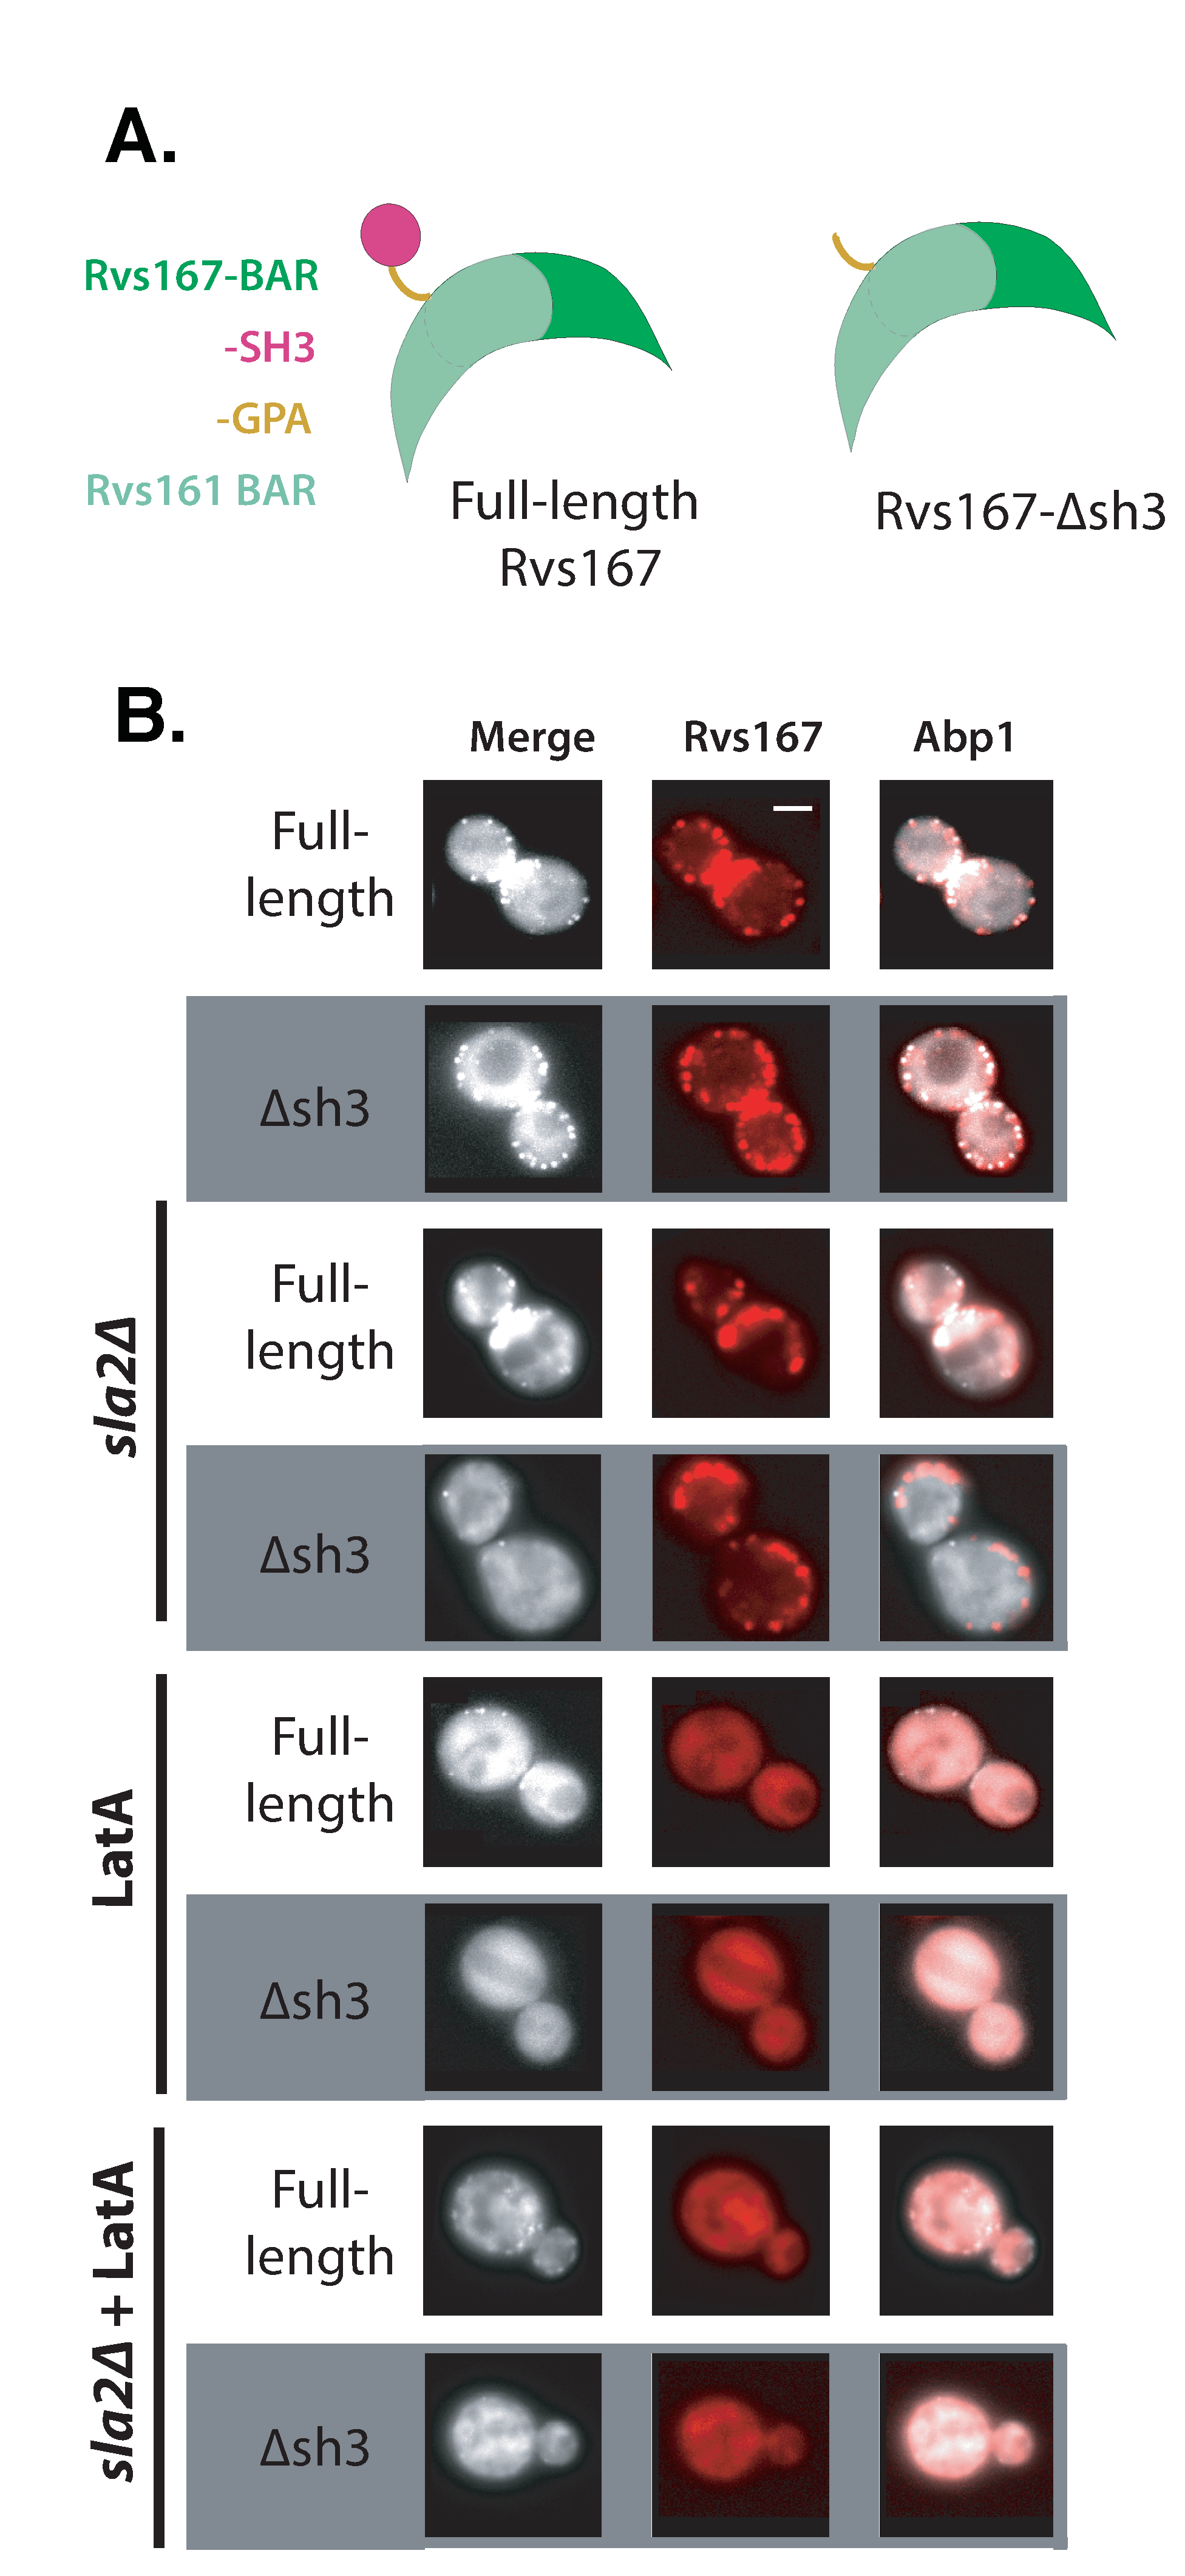
\includegraphics
	[width=0.45\hsize]{/Users/deepikaa/Desktop/scission_paper/figures/fig3/sla2_del_final16.pdf}
	\caption{\textbf {Localization of Rvs167 BAR domain} 
		\textbf{A:} Schematic of Rvs protein complex with and without the SH3 domain.  \textbf{B:} Localization of full-length Rvs167 and Rvs167\textit{$\Delta$sh3} in WT, \textit{sla2$\Delta$}, LatA treated, and LatA treated \textit{sla2$\Delta$} cells. Scale bar=2{\textmu}m.}
	\label{sla2del}
\end{figure}

So far Rvs167 remains the protein that has a major influence on scission efficiency and movement of Sla1. Rvs can tubulate liposomes in vitro \citep{Youn2010}, but its interaction with membrane curvature in vivo has not so far been tested.  Recruitment of the Rvs complex to endocytic sites, and BAR-membrane interaction was thus investigated further. The SH3 domain has known interactions with proteins within actin network \citep{Lila1997,Colwill1999,Madania1999,Liu2009}. We removed the contribution of the SH3 by deleting the domain (Fig.\ref{sla2del}A) and observed the localization of Rvs167\textit{$\Delta$sh3} compared to full-length Rvs167. Endogenously tagged Rvs167-eGFP and Rvs167\textit{$\Delta$sh3}-eGFP colocalization with Abp1-mCherry in WT and \textit{sla2$\Delta$} cells were compared (Fig.\ref{sla2del}B). Sla2 acts as the molecular linker between forces exerted by the actin network and the plasma membrane \citep{Skruzny2012}. \textit{sla2$\Delta$} cells therefore contain a polymerizing actin network at endocytic patches, but the membrane has no curvature, and endocytosis fails. In these cells, the full-length Rvs167 co-localizes with Abp1-mCherry, indicating that it is recruited to endocytic sites independently of membrane curvature (Fig.\ref{sla2del}B, “\textit{sla2$\Delta$}”). Rvs167\textit{$\Delta$sh3} does not localize to the plasma membrane except for rare transient patches that do not co-localize with Abp1-mCherry: Rvs167\textit{$\Delta$sh3} is not recruited to endocytic sites in the absence of curvature in \textit{sla2$\Delta$} cells.


\subsection{Rvs SH3 domains have an actin and curvature independent localisation}
In order to test if genetic interactions of SH3 domains are prevalent in in vivo endocyotosis, we tested the localization of Rvs167 and Rvs167textit{$\Delta$sh3} in LatA treated cells (Fig.\ref{sla2del}B, “LatA”). Plasma membrane localization of Rvs167 remains upon LatA treatment, and transient patches continue to exist in \textit{sla2$\Delta$} cells treated with LatA (Fig3B, “\textit{sla2$\Delta$}+ LatA”). Rvs167textit{$\Delta$sh3} does not localize to the plasma membrane in either case. Thus, localization of full-length Rvs167 in the presence of LatA is due to the SH3 domain. This indicates that the SH3 domain is able to recruit Rvs molecules to the plasma membrane in an actin- and curvature-independent manner. 

%DISCUSSION {Rvs SH3 domains contribute to curvature independent localization}
%We have shown that yeast N-BAR domains need membrane curvature to localize in vivo. Full-length Rvs167, however, is recruited to endocytic patches in \textit{sla2$\Delta$} cells. This indicates that a second interaction- that is not the BAR-curvature dependent- recruits the protein to endocytic sites. This interaction must come from the SH3 region, showing that Rvs localization is dependent on both BAR as well as SH3 domain interactions. Absence of the SH3 domain also reduces total recruitment of Rvs and Abp1 protein, giving the SH3 domain an important and surprising role in regulating the late stage of endocytosis. 



\subsection{SH3 domains are likely recruited by Myosin 3}
Type I myosins Myo3 and Myo5, and Vrp1 have known genetic and/or physical interactions with Rvs167 SH3 domains \citep{Lila1997,Colwill1999,Madania1999,Liu2009}. We tested the interaction between these proteins and the Rvs167 SH3 region by studying the localization of full-length Rvs167 in cells with one of the genes for these proteins deleted, and treated with LatA. By using LatA we expected to reproduce the situation in which BAR-curvature interaction is removed (Fig.\ref{sh3_loc}B). Then, if we lost SH3 interaction because we removed the protein with which it interacts, we would lose localization of Rvs167 completely. Deletion of neither Vrp1 nor Myo5 in combination with LatA treatment removes the localization of Rvs167. Deletion of Myo3 with LatA treatment removes localization of Rvs167, indicating that SH3 domains interact at endocytic sites with Myo3.

\begin{figure}[h]
	\centering
	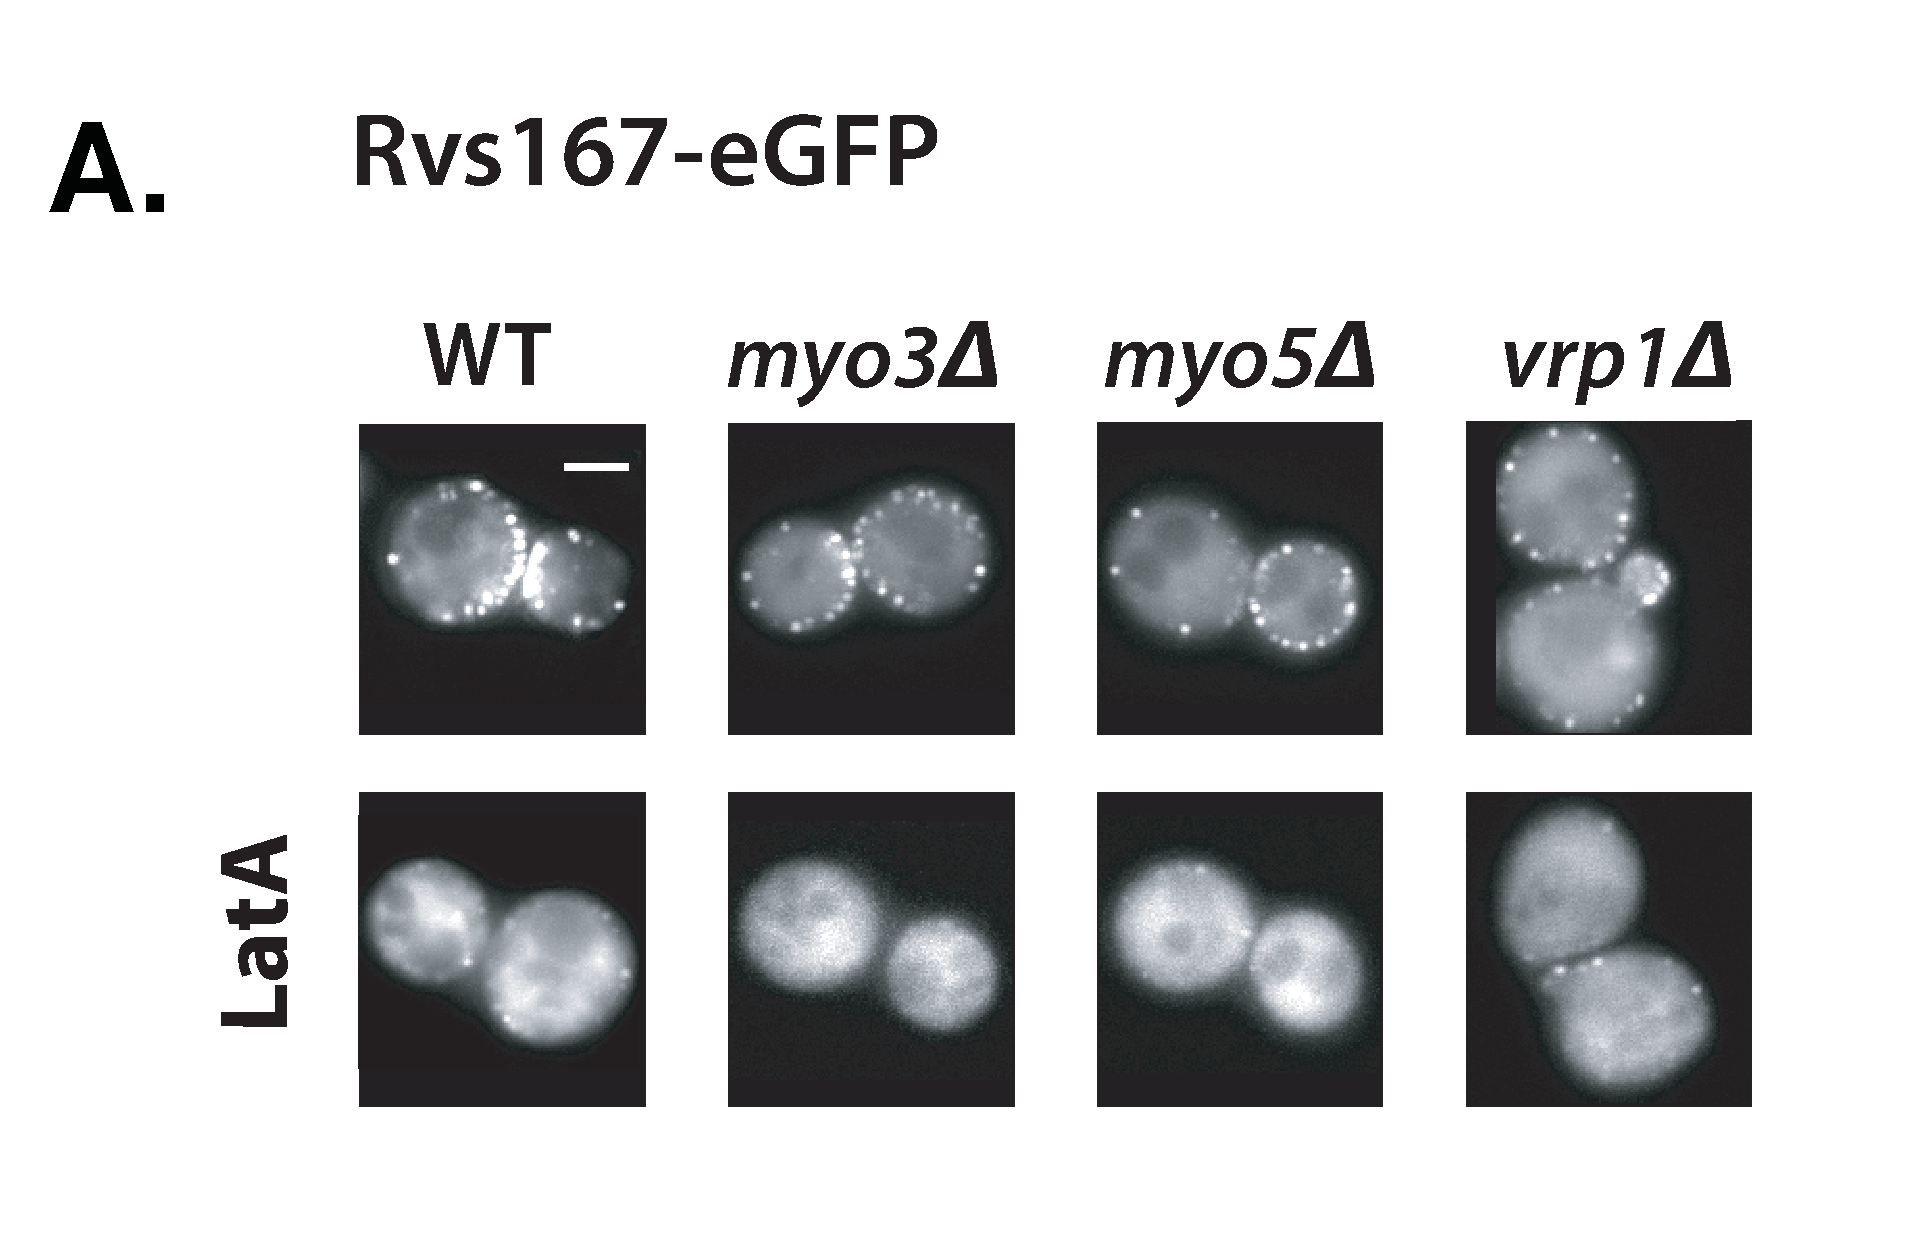
\includegraphics
	[width=0.4\hsize]{/Users/deepikaa/Desktop/scission_paper/figures/fig3/fig3_sh3loc.pdf}
	\caption{ \textbf {Localization of the SH3 domain}
Localization of full-length Rvs167-eGFP in WT, \textit{myo3$\Delta$}, \textit{myo5$\Delta$}, and \textit{vrp1$\Delta$} cells. Scale bars=2{\textmu}m.}
	\label{sh3_loc}
\end{figure}

\subsubsection{\color{red} 
	what about the differences in myo5 and myo3 number... 
}

\subsection{Loss of Rvs167 SH3 domain affects coat and actin dynamics}
Since the Rvs167 SH3 domain has an influence on the recruitment of the Rvs complex to endocytic sites, we wondered if the domain also affects later stages of invagination formation endocytic dynamics. We compared dynamics of coat and scission markers in WT and \textit{rvs167$\Delta$sh3} cells (Fig.\ref{delsh3}). Movement of Sla1 centroid is slower and reduced in \textit{rvs167$\Delta$sh3} cells compared to WT (Fig4A,B). The movement of Rvs167textit{$\Delta$sh3}  centroid is smaller than that of full-length Rvs167 (Fig.\ref{delsh3}A,B), consistent with the formation of shorter invaginations suggested by the reduced Sla1 movement in \textit{rvs167$\Delta$sh3} cells.
\begin{figure}[h]
	\centering
	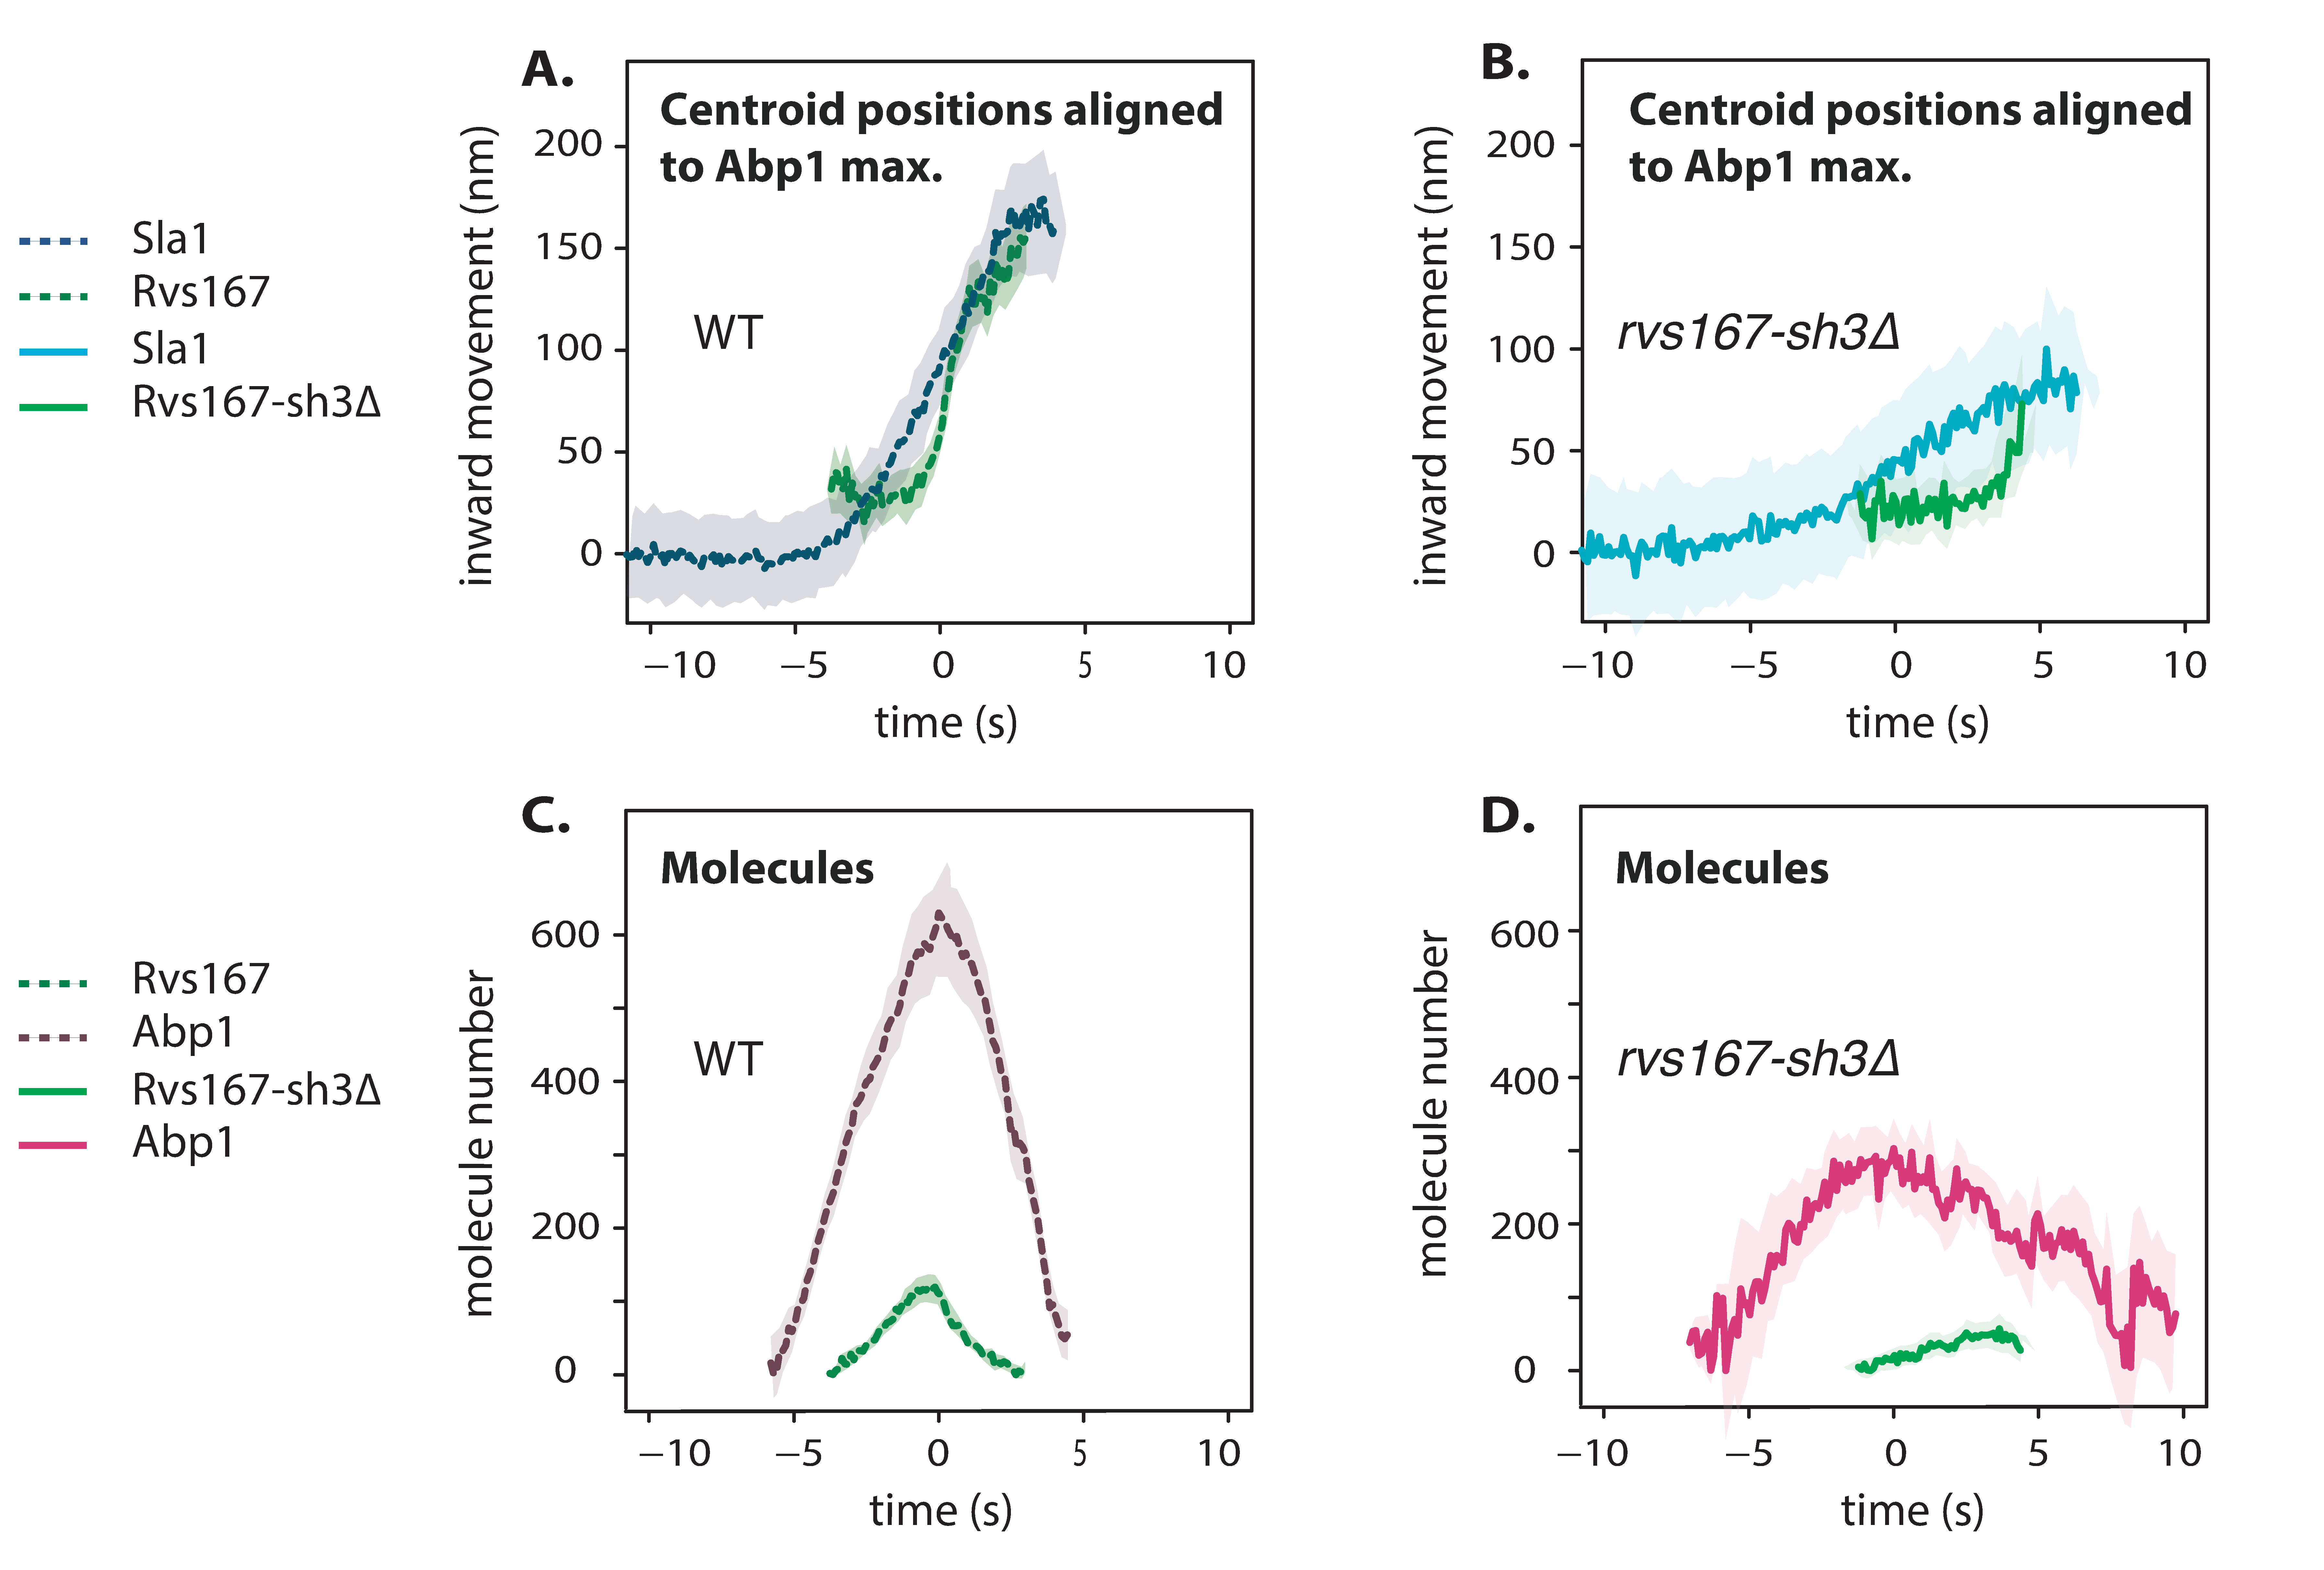
\includegraphics
	[width=0.75\hsize]
	{/Users/deepikaa/Desktop/scission_paper/figures/fig4/delsh3_9.pdf}
	\caption{\textbf {Endocytic dynamics in \textit{rvs167$\Delta$sh3} cells} 
		\textbf{A,B:} Averaged centroid positions aligned in x axis so that time=0(s) is the peak of fluorescent intensity of Abp1 in respective strains. Centroids are aligned in y axis so that Sla1 begins at y=0 (nm), and Rvs167 and Rvs167\textit{$\Delta$sh3} positions are determined with respect to Sla1 centoids. \textbf{C,D:} Numbers of molecules of in WT and \textit{rvs167$\Delta$sh3} cells, aligned so that time=0(s) is the maximum of fluorescent intensity of Abp1 in the corresponding strains.}
	\label{delsh3}
\end{figure}


There is delay in Rvs167\textit{$\Delta$sh3} recruitment compared to the onset of Abp1 assembly in \textit{rvs167$\Delta$sh3} cells compared to WT (Fig.\ref{delsh3} C,D). In WT cells, Rvs167 and Abp1 molecule number peaks are also coincident: the actin network begins disassembling as soon as scission occurs (Fig.\ref{delsh3}C). Asynchronous peaks in \textit{rvs167$\Delta$sh3} cells indicates a disruption in the feedback between actin network dynamics and membrane scission. Rvs167textit{$\Delta$sh3} accumulation begins however, when Abp1 molecule numbers in the mutant are about the same as in WT (about 300 copies, Fig.\ref{delsh3}C,D). . Both Rvs167 and Rvs167\textit{$\Delta$sh3} molecules arrive at endocytic sites when the Sla1 centroid is 20-30 nm away from its starting position. This would mean the endocytic coat has moved about 30 nm when both WT and mutant forms of Rvs are recruited. That Rvs167\textit{$\Delta$sh3} recruitment anticipates a certain growth of the invagination and amount of Abp1 suggests that the Rvs complex is recruited to a specific geometry of membrane invagination, and that Rvs167\textit{$\Delta$sh3} recruitment is delayed because invaginations in these cells take longer to acquire this specific geometry. Recruitment of Rvs167\textit{$\Delta$sh3}  is reduced to half of Rvs167 (Fig.\ref{delsh3}C,D), although cytoplasmic concentration of both are similar (Fig.\ref{delsh3_cytoplasmic}). Recruitment therefore is unlikely to be limited by cytoplasmic expression of the mutant protein. Abp1 disassembly is slowed down in \textit{rvs167$\Delta$sh3} cells compared to WT, and recruitment is reduced to 50\% of WT recruitment (Fig.\ref{delsh3}C,D), indicating disruption of actin network dynamics.

%\subsection{N-helix and GPA domains do not contribute to recruitment of Rvs or membrane movement}
%\lipsum[12]
	
%\subsection{Reduced BAR domain recruitment corresponds to reduced membrane movement}
\subsection{Increased BAR domain recruitment corresponds to increased membrane movement}
Since removal of Rvs167 in \textit{rvs167$\Delta$sh3}  cells, and the reduced amount of Rvs167\textit{$\Delta$sh3}  recruited in \textit{rvs167$\Delta$sh3} cells results in decreased Sla1 movement, we wondered if Sla1 movement would scale with amount of Rvs recruited to endocytic sites. We titrated the amount of Rvs expressed in cells by endogenously duplicating the Rvs167 and Rvs161 genes (Huber et al. 2014) in diploid and haploid yeast cells (Fig.5) . We thus made diploid strains with 4x copies of both the Rvs genes (4xRVS), 2x copies (WT diploid cells, 2xRVS), and 1x copy (1xRVS). Number of molecules of Rvs167 recruited to endocytic sites increases with gene copy number (Fig5A). “Excess” Rvs recruited to endocytic sites in the 4xRVS case does not change the rate or total movement of Sla1, or of Rvs167 (Fig.\ref{duplication}B,C) compared to the WT (2xRVS). In the case of 1xRVS, Sla1 movement is slightly reduced after 100nm (Fig.\ref{duplication}B). Magnitude of Rvs167 inward movement was similar in all three, but the Rvs167-eGFP signal was lost immediately after the inward movement in the 1xRVS case, unlike in the 4xRVS and 2xRVS cases, likely because fewer molecules are recruited (Fig.\ref{duplication}A). Unlike in the \textit{rvs167$\Delta$sh3}  case, Abp1 and Rvs167 peaks were concomitant in all three strains, with similar amounts of Abp1 recruited irrespective of Rvs gene copies (Fig.\ref{duplication}D). Thus was there no apparent disruption of the actin network, or of the coupling between scission and actin network disassembly. Adding more Rvs than in the WT diploid case did not lead to differences in Sla1 movement, although reducing the amount of Rvs- as in the 1xRVS case- marginally decreased movement. 

In haploid cells, we duplicated the full-length Rvs167 gene, as well as \textit{rvs167$\Delta$sh3} gene (Fig5E-H). We thus produced strains with 2x copies of the Rvs genes (2xRVS), 1x copy of each (WT haploid, 1xRVS), 2x copies of the \textit{rvs167$\Delta$sh3} gene (2xBAR), or 1 copy of \textit{rvs167$\Delta$sh3} gene (1xBAR). Amount of WT and mutant Rvs167 molecules recruited at endocytic sites varied in these strains between 50 and 180 copies (Fig5E). Sla1 dynamics remained the same in Rvs duplicated strain (2xRVS) as in the WT (Fig.\ref{duplication}F). In the 2xBAR case, the amount of Rvs167\textit{$\Delta$sh3}  molecules  recruited to endocytic sites increased (Fig.\ref{duplication}E), as did Sla1 movement, as well the inward jump of Rvs167 (Fig.\ref{duplication}F,G), compared to 1xBAR. Total Abp1 numbers recruited were reduced in 1xBAR (that is \textit{rvs167$\Delta$sh3}), compared to the 2xBAR, 1xRVS and 2xRVS (Fig5H). Higher Abp1 numbers corresponds to larger Sla1 centroid movement in both diploid and haploid cells (Fig.\ref{duplication}C, D, G, H), suggesting a correlation between the maximum number of Abp1 recruited and total invagination length.




\begin{figure}[h]
	\includegraphics[
	width=1.0\textwidth,
	height=1.0\textwidth,
	keepaspectratio=true
	] {/Users/deepikaa/Desktop/scission_paper/figures/fig5/fig5_7.pdf}
	\caption{\textbf {RVS duplication in haploid and diploid cells} 
	\textbf{A:} Recruitment of Rvs167 in diploid strains with different copy number of Rvs167 and Rvs161 genes. \textbf{B:} Rvs167 centroid positions in these strains \textbf{C:} Sla1 centroid positions in these strains. \textbf{D:} Abp1 molecule numbers in same strains, with only one Abp1 allele tagged. 
	\textbf{E,F:} Recruitment and centroid positions of Rvs167 and Rvs167\textit{$\Delta$sh3} in haploid strains.  \textbf{G:} Sla1 centroid positions in these strains. \textbf{H:} Abp1 recruitment in the same strains. All centroid positions were aligned in the time axis so that time=0(s) corresponds to beginning of inward movement of each average centroid. Centroids were aligned in the y axis so that y=0(nm) corresponds to the beginning of the average centroid position}
	\label{duplication}
\end{figure}


%\begin{table}[bt]
%\caption{\label{tab:example}Automobile Land Speed Records (GR 5-10).}
% Use "S" column identifier to align on decimal point 
%\begin{tabular}{S l l l r}
%\toprule
%{Speed (mph)} & Driver          & Car                        & Engine    & Date     \\
%\midrule
%407.447     & Craig Breedlove & Spirit of America          & GE J47    & 8/5/63   \\
%413.199     & Tom Green       & Wingfoot Express           & WE J46    & 10/2/64  \\
%434.22      & Art Arfons      & Green Monster              & GE J79    & 10/5/64  \\
%468.719     & Craig Breedlove & Spirit of America          & GE J79    & 10/13/64 \\

%\end{tabular}

%\medskip 
%Source: \url{https://www.sedl.org/afterschool/toolkits/science/pdf/ast_sci_data_tables_sample.pdf}

%\tabledata{This is a description of a data source.}

%\end{table}


\section{Discussion}
Recruitment and function of the Rvs complex has been studied in this work, and several existing models for membrane scission have been tested. We propose that Rvs is recruited to endocytic sites via interactions between the Rvs BAR domains and invaginated membrane, and that SH3 mediated protein-protein interactions are required for efficient recruitment of Rvs. We found that arrival of Rvs at the membrane invagination scaffolds the membrane and prevents membrane scission. WT invagination lengths depend on recruitment of a critical number of Rvs molecules. Both timing and recruitment efficiency appear crucial to Rvs function.

\subsection{BAR domains sense \textit{in vivo} membrane curvature and time recruitment of Rvs}
The curved structure of Endophilin and Amphiphysin BAR dimers \citep{Peters2004,Mim2012} In the absence of membrane curvature- in \textit{sla2$\Delta$} cells- Rvs167\textit{$\Delta$sh3} domains do not localize to endocytic sites (Fig.\ref{delsh3}B). This demonstrates for the first time that the BAR domain senses and requires membrane curvature to localize to endocytic sites. Rvs167\textit{$\Delta$sh3} has a similar average lifetime at endocytic sites as full length Rvs167 (Fig.\ref{delsh3}C,D). However, time alignment with Abp1 shows that there is a delay in the recruitment of Rvs167\textit{$\Delta$sh3} (Fig.\ref{delsh3}B). Sla1
moves inwards at a slower rate in bar-gpa cells, so it takes longer for the membrane in these cells to reach the same invagination length as in WT. We propose that Rvs recruitment is timed to specific membrane invagination length- therefore to a specific membrane curvature \-/  accounting for the delay in recruitment. The timing of recruitment is therefore provided by the BAR domain. 


%has suggested that Rvs is recruited by its preference for some membrane shapes over others, supported by its arrival at curved membrane tubes. In the absence of membrane curvature, in  \textit{sla2$\Delta$}  cells, the BAR domain alone does not localize to cortical patches (Fig.3b,c). This demonstrates for the first time that the BAR domain does indeed sense and requires membrane curvature to localize to cortical patches. Work on BAR domains have proposed that electrostatic interactions at the concave surface and tips of the BAR domain structure mediate membrane binding \cite{Qualmann2011}. Mutations in these lipid-binding surfaces would clarify the interaction with underlying lipids, and test if Rvs relies on similar interactions.
%BAR is able to localize to endocytic sites, and has a similar lifetime in WT cells (Fig4b). However, time alignment with Abp1 shows that there is a delay in the recruitment of BAR-GPA compared to Abp1 arrival, compared to full-length Rvd167 (Fig4c). The delayed recruitment occurs because the invagination takes longer to reach a particular length: Sla1 moves inwards at a slower rate in BAR cells, and it takes longer for the membrane in BAR-GPA cells to reach the same length as Rvs167. Rvs167 arrives in BAR cells when Sla1 has moved inwards 25-30nm (dashed red lines in Fig.4a), which is also the distance Sla1 has moved when Rvs167 arrives in WT. By the time Sla1 has moved this distance, the membrane is already tubular (Kukulski et al., 2012; Picco et al., 2015), consistent with Rvs arrival at invaginated tubes. This suggests Rvs recruitment is timed to specific membrane invagination length- therefore to a specific membrane curvature- and that this timing is provided by the BAR domain.

%In Fig.3.3.3B we see that while the full-length Rvs167 arrives about 4 seconds after the arrival of Abp1, BAR arrives only 6 seconds after Abp1 arrives. There is a time delay between Abp1 recruitment and BAR arrival, compared to the arrival of full-length Rvs167, confirmed by the TIRF measurement in 3.3.3D. The delay in recruitment could occur because the membrane has not acquired the required invagination length or because the loss of the SH3 domain causes delayed recruitment. That the delayed recruitment occurs because the invagination takes longer to reach a particular length is supported by the fact that Sla1 moves inwards at a slower rate in BAR cells. It takes longer for the membrane in BAR cells to reach the same length as WT. Rvs167 arrives in BAR cells when Sla1 has moved inwards 25-30nm (dashed red lines in Fig.3.3.3A), which is also the distance Sla1 has moved when Rvs167 arrives in WT. By the time Sla1 has moved this distance, the membrane is already tubular (Kukulski et al., 2012; Picco et al., 2015), consistent with Rvs arrival at invaginated tubes. This suggests Rvs recruitment is timed to specific membrane invagination length- therefore to a specific membrane curvature- and that this timing is provided by the BAR domain.

\subsection{SH3 domains allow efficient and actin independent recruitment}

\textit{Rvs167$\Delta$sh3} accumulates to about half the WT number (Fig.\ref{delsh3}C,D), even though the same cytoplasmic concentration is measured (Fig.\ref{delsh3} supplement), indicating that loss of the SH3 domain decreases the efficiency of recruitment of Rvs. In \textit{sla2$\Delta$} cells, full-length Rvs167 forms patches on the membrane (Fig.\ref{sla2del}B). Since Rvs167\textit{$\Delta$sh3} does not localize to the plasma membrane in \textit{sla2$\Delta$} cells, localization of the full-length protein must be mediated by the SH3 domain. That full-length Rvs167 is able to assemble and disassemble at cortical patches in \textit{sla2$\Delta$} cells without the curvature- dependent interaction of the BAR domain (Fig.\ref{sla2del}B) indicates that the SH3 domain can mediate both the recruitment and disassembly of Rvs at endocytic sites. In \textit{sla2$\Delta$} cells treated with LatA (Fig.\ref{sla2del}B), both membrane curvature and actin-interacting proteins are removed from endocytic sites. Full-length Rvs167 in these cells still shows transient localizations at the plasma membrane: the SH3 domain is able to localise the Rvs complex in an actin and curvature independent manner. 


\subsection{Loss of SH3 domain disrupts endocytic actin network dynamics}
In WT cells, the Abp1 and Rvs167 fluorescent intensities reach maxima concomitantly (Fig.\ref{delsh3}C,D), and the consequent decay of both coincide. Coincident disassembly indicates that upon vesicle 
scission, the actin network is immediately disassembled. Membrane scission occurs around the intensity peak of the two proteins \citep{Kukulski2012,Picco2015}. This coincident peak is lost in bar-gpa cells: Rvs167\textit{$\Delta$sh3} average fluorescent intensity peaks several seconds after Abp1 intensity starts to drop, and the decay of 
Abp1 is prolonged, taking nearly double the time as in WT. Although it is not clear what the decoupling of 
Abp1 and Rvs167\textit{$\Delta$sh3} peaks means, the changes in Abp1 dynamics suggests a strong disruption of the actin
network dynamics.


\subsection{Rvs acts as a membrane scaffold preventing membrane scission}
Invaginations in \textit{rvs167$\Delta$} cells undergo scission when the Sla1 centroid has moved about 80nm (Fig.\ref{vps}F), compared to the WT lengths of 140nm. This shows that enough forces are generated at 80nm to cause scission. Since invagination lengths of \textit{rvs167$\Delta$} cells are increased by overexpression of the Rvs167\textit{$\Delta$sh3} domains (Fig.\ref{duplication}E-G), we think that localization of Rvs BAR domains to the membrane tube stabilizes the  membrane \citep{Boucrot2012,Dmitrieff2015} This allows the invagination to grow until actin polymerization produces enough forces to sever the membrane. The requirement for Rvs scaffolding cannot be removed by reducing turgor pressure (Fig.\ref{duplication}supplement? or 7?),  so the function of the scaffold is not to counter turgor pressure. There is a limit to the stabilizaiton by BAR domains: in diploid strains with 4 copies of each RVS gene, the same amount of actin is recruited before scission. The invaginations lengths are the same as in the other strains even though more Rvs is recruited. It is possible that the nature of the Rvs complex interaction with the membrane changes after a certain amount of Rvs is recruited. 

If enough forces are generated at 80nm, why is scission efficiency decreased in \textit{rvs167$\Delta$}  compared to WT? Forces from actin may be at a threshold when the invagination is at 80nm. There could be enough force to sever the membrane, but not enough to sever reliably. The Rvs scaffold then keeps the network growing to accumulate enough actin to reliably cause scission. Controlling membrane  tube length could also be a way for the cell to control the size of the vesicles formed, and therefore the amount of cargo packed into the vesicle. 

\subsection{What causes membrane scission?}
We looked for changes in the dynamics of Sla1 and Rvs167 that would indicate a scission defect in various mutant strains: longer invaginations than in WT, so Sla1 centroid movements of over 140nm, and a bigger inwards jump of Rvs167 centroid, indicating that a longer invagination has been cut. In \textit{vps1$\Delta$}  cells, no major changes are seen in Sla1 or Rvs167 dynamics. We conclude that even if Vps1 is recruited to endocytic sites, it is not necessary for Rvs localization or function, and is not necessary for scission. 

In the lipid hydrolysis model, synaptojanins hydrolyze PIP\textsubscript{2}  molecules that are not covered by BAR domains, resulting in a boundary between hydrolyzed and non- hydroplyzed PIP\textsubscript{2}. Interfacial forces generated at this lipid boundary causes scission \citep{Liu2006}. Deleting  synaptojanins Inp51 and Inp52 should increase invagination lengths if scission was driven by lipid hydrolysis. Sla1 and Rvs centroid dynamics shows that deletion of neither Inp51 nor Inp52 result in scission delay. In \textit{inp51$\Delta$}  cells, Rvs assembly is slightly slower than that in WT: Inp51 could play a role in Rvs recruitment. In the \textit{inp52$\Delta$}  strain, about 12\% of Sla1-GFP tracks retract, this could suggest a moderate influence of Inp52 on scission. Rvs centroid persists after scission in \textit{inp52$\Delta$}  cells: disassembly of Rvs after scission is delayed. Sla1 signal also persists for longer after scission in the \textit{inp52$\Delta$} than in WT cells, suggesting that post-scission disassembly of proteins from the vesicle is inhibited in \textit{inp52$\Delta$}  cells. Inp52 likely plays a role in recycling endocytic proteins from the vesicle to the plasma membrane. 

A protein-friction model has proposed that BAR domains induce a frictional force on the membrane, causing scission (ref!). If more BAR domains were added to the membrane tube at a faster rate, the frictional  force generated as the membrane is pulled under it should increase, and the membrane should rupture faster. That is, membrane scission should occur as soon as WT forces are generated on the tube. In Rvs duplicated cells, adding up to 1.6x the WT amount of Rvs at faster rates to membrane tubes does not affect the length at which the membrane undergoes scission (Fig.\ref{duplication}E). We think that protein friction does not contribute significantly to membrane scission in yeast endocytosis. 

~\\
We  observed that the maximum amount of Abp1 measured in all the diploid strains is about 220 molecules (Fig.\ref{duplication}D). Since only one allele of Abp1 is fluorescently tagged in these strains, the total amount of Abp1 recruited is  about 440±20 molecules. In WT haploid cells, the maximum number of Abp1 measured is 460±20 molecules. We propose that recruitment of a similar amount of Abp1 before scission in all these strains indicates that scission is dependent on the amount of Abp1, and correspondingly, on the amount of actin recruited. We propose that actin supplies the forces necessary for membrane scission. The membrane invagination continues until the “right” amount of actin is recruited. The amount of force necessary is determined by the physical properties of the membrane like membrane rigidity, tension, and proteins accumulated on the membrane \citep{Dmitrieff2015}. Vesicle scission releases membrane-bound Rvs, resulting in release of the SH3 along with BAR domains. Release of the SH3 domains could indicate to the actin network that vesicle scission has occurred, beginning disassembly of actin components. 


\subsection{Model for membrane scission}
We propose that Rvs is recruited to sites by two distinct mechanisms. SH3 domains cluster Rvs at endocytic sites, increasing the efficiency with which the BAR domains sense curvature on tubular membranes. BAR domains bind to endocytic sites by sensing tubular membrane. Membrane shape is stabilized by BAR-membrane interaction against fluctuations that could cause scission. This prevent actin forces from rupturing the membrane, and the invaginations continue to grow in length as actin continues to polymerize. As actin continues to polymerize,, enough forces are generated to overcome the resistance to membrane scission provided by the BAR scaffold. The membrane ruptures, and vesicles are formed. Synaptojanins may help recruit Rvs at endocytic sites: Inp51 and Inp52 have proline rich regions that could act as binding sites for Rvs167 SH3 domains. They are involved in vesicle uncoating post-scission, likely by dephosphorylating PIP\textsubscript{2} and inducing disassembly of PIP\textsubscript{2} -binding endocytic proteins. Eventually phosphorylation regulation allows endocytic proteins to be reused at endocytic sites, while the vesicle is transported elsewhere into the cell. 


%Fig.4C shows that recruitment of BAR is reduced to half that of Rvs167 (57±9.9 for BAR compared to 113.5±5.3 for Rvs167). Cytoplasmic concentration of Rvs167 and BAR are not different (supplement). The inward jump of BAR is less than that of full-length Rvs167 (Fig.4A). 
%DISCUSSIONThis indicates that although the BAR is expressed at the same level at WT Rvs167, it is recruited less efficiently. The inward jump of BAR is less than that of full-length Rvs167 (Fig.3.4A). The decrease in inward jump indicates that the position of the newly formed vesicle in BAR cells is lower than in WT. This would imply that invagination lengths are reduced in BAR cells compared to WT.
%We have shown that yeast N-BAR domains need membrane curvature to localize in vivo. Full-length Rvs167, however, is recruited to endocytic patches in \textit{sla2$\Delta$} cells. This indicates that a second interaction- that is not the BAR-curvature dependent- recruits the protein to endocytic sites. This interaction must come from the SH3 region, showing that Rvs localization is dependent on both BAR as well as SH3 domain interactions. Absence of the SH3 domain also reduces total recruitment of Rvs and Abp1 protein, giving the SH3 domain an important and surprising role in regulating the late stage of endocytosis. 
%DISCUSSION
%This delay in decrease of Sla1-GFP signal is consistent with delay in vesicle uncoating rather than membrane scissison. 
%Rvs: Similarly, indicating a delay in removing endocytic proteins from the newly formed vesicle. Assembly of Rvs167 has a delay in \textit{inp51$\Delta$} cells , which could indicate a defect in recruiting proteins to endocytic sites, or in progression of endocytic invaginations. Since Sla1 movement is the same, we suggest a defect in the former rather than latter. 

%\begin{figure}
%			\hspace*{-1cm}
%				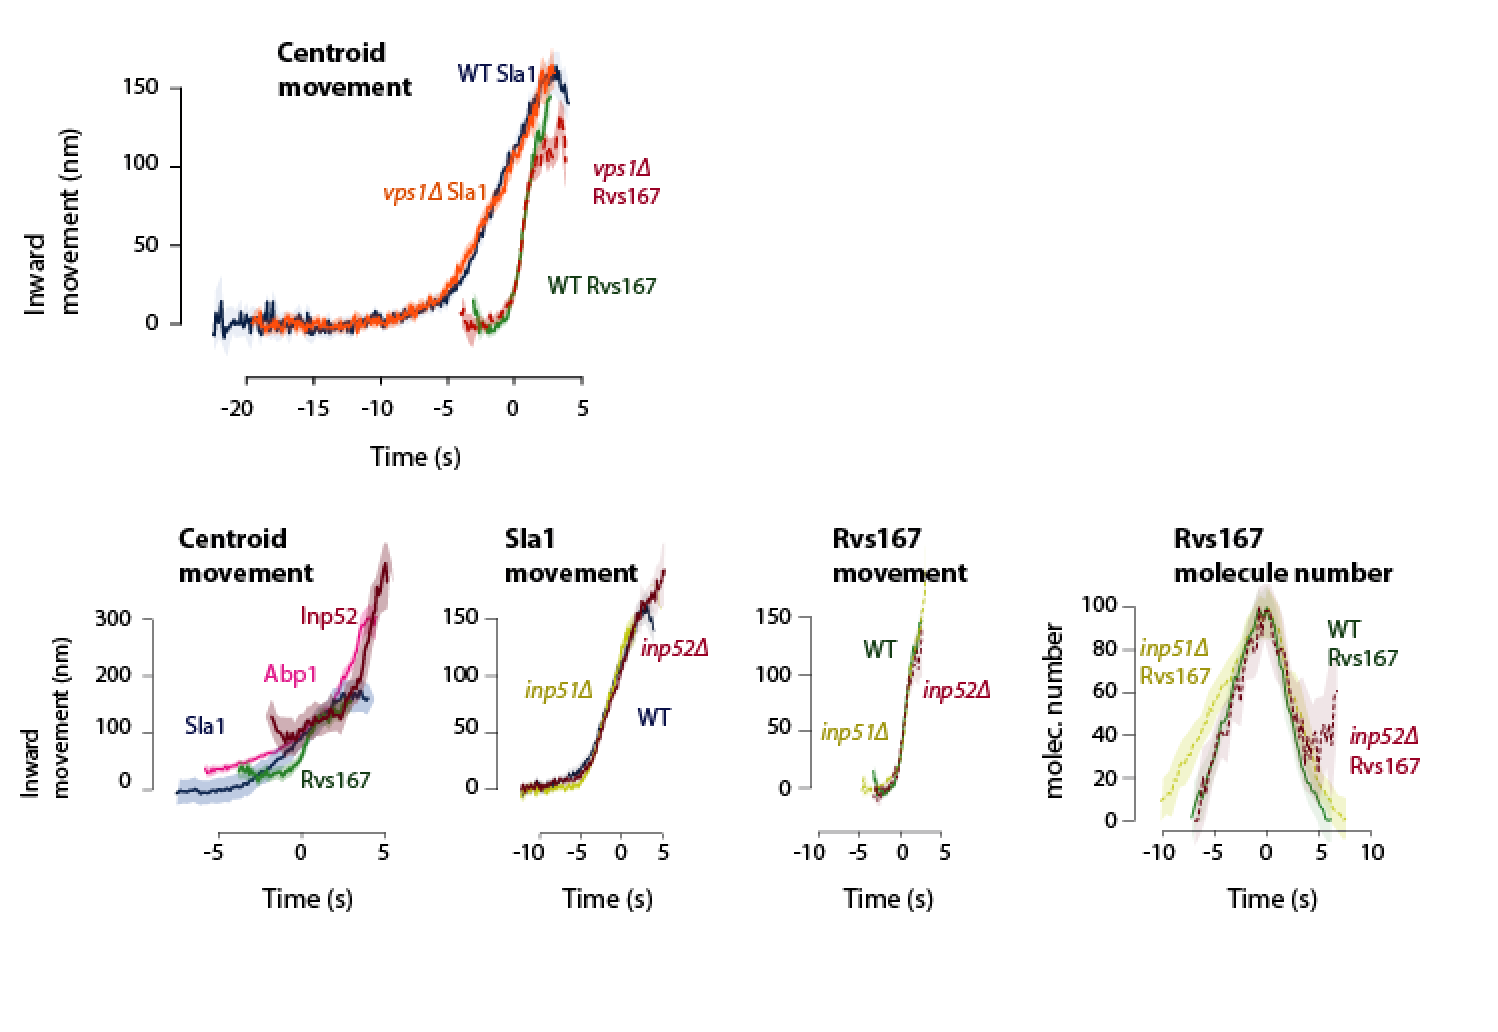
\includegraphics[width=4cm, height=4cm, keepaspectratio]{figures/vps1_placeholder}
%	\caption[Endocytic pathways in cells]
%			\label{intro_mayor}}
%\end{figure}

%\begin{wrapfigure}{l}{.46\textwidth}
%	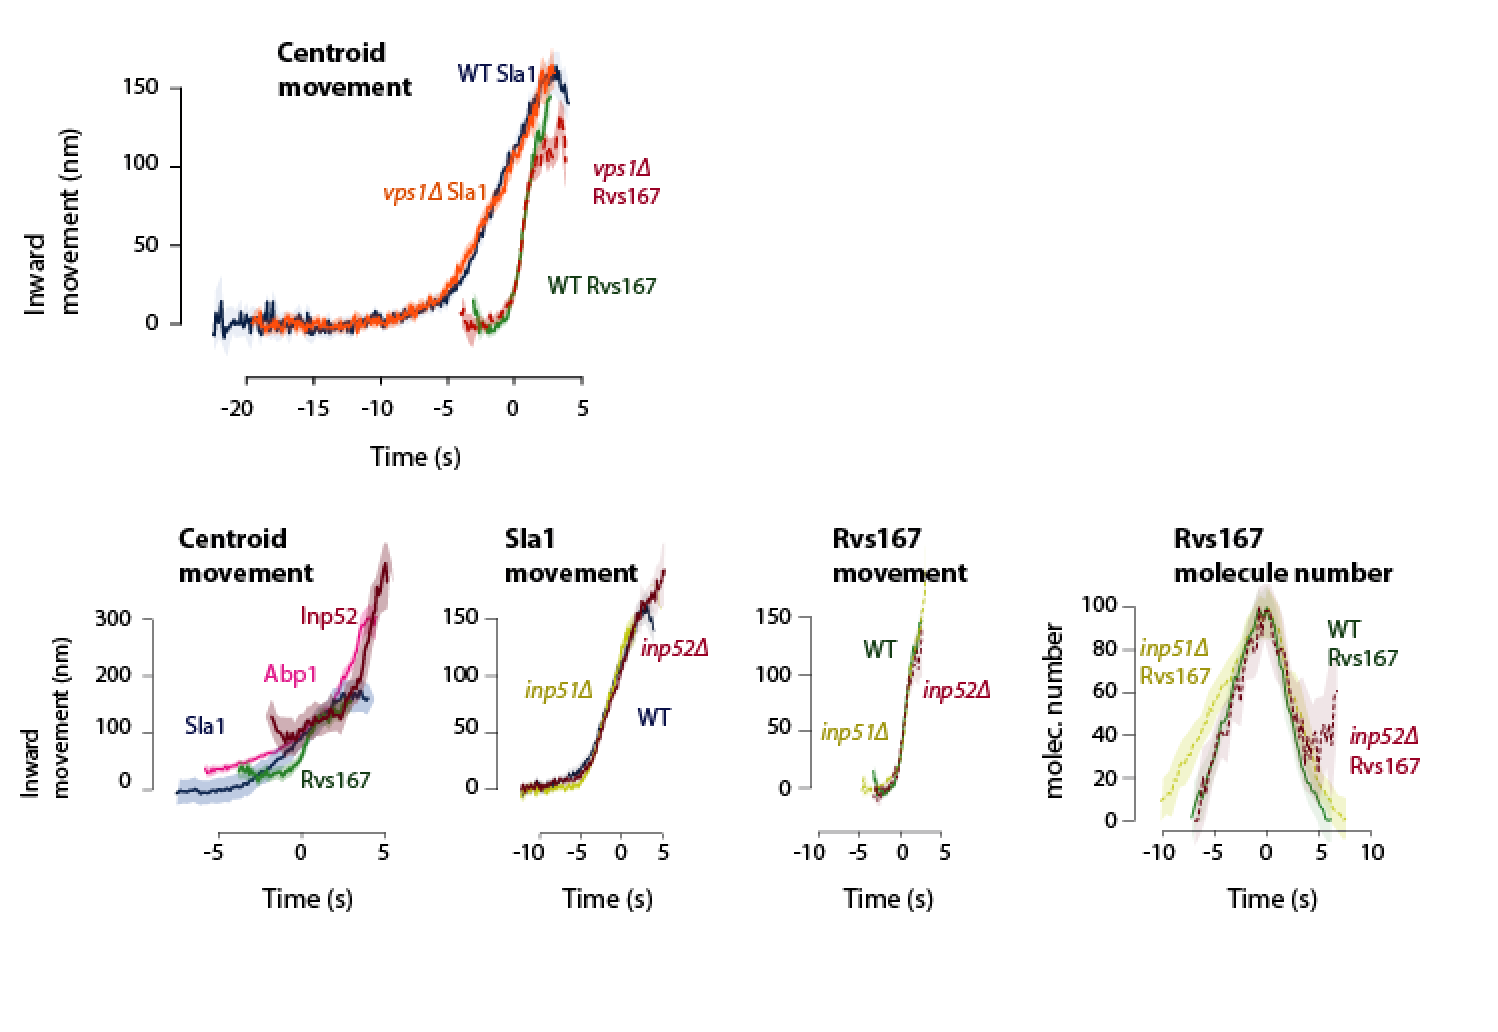
\includegraphics[width=\hsize]{figures/vps1_placeholder}
%	\caption{A half-columnwidth image using wrapfigure, to be used sparingly. Note that using a wrapfigure before a sectional heading, near other floats or page boundaries is not recommended, as it may cause interesting layout issues. Use the optional argument to wrapfigure to control how many lines of text should be set half-width alongside it.}
%	\label{fig:halfwidth}
%\end{wrapfigure}



\section{Methods and Materials}

\subsection{Homologous recombination with PCR casette in- sertion}
Tagging or deletion of endogenous genes was done by homologous integration of the product of a Polymerase Chain Reaction using appropriate primers and a plasmid containing a selection cassette and fluorescent tag, or only selection cassette for gene deletions. Primers were designed according to Janke et al, 2004. PCRs used the Velocity Polymerase for fluorescent tagging, and Q5 for gene deletions using the NAT casette. All fluorescently tagged genes have a C-terminus tag and are expressed endogenously. Gene deletions and fluorescent tags are checked by PCR. Vps1del and gene duplications were confirmed by sequencing.


\subsection{Live-cell imaging and electron microscopy}
\subsubsection{Sample preparation for live imaging}
40{\textmu}L Concavalin A (ConA) was incubated on a coverslip for 10 minutes. 40{\textmu}L Yeast cells incubated overnight at 25C in imaging medium SC-TRP was added to the coverslip after removing the ConA, and incubated for another 10 minutes. Cells were then removed, adhered cells were washed 3x in SC-TRP, and 40{\textmu}L SC-TRP was finally added to the coverslip to prevent cells from drying.

\subsubsection{Sample preparation for live imaging in LatA and sorbitol treated cells}
Cells went through the same procedure as above till the last washing step. Instead of SC-TRP, 100x diluted LatA, or Sorbitol at a final concentration of 0.2M in SC-TRP was added to the adhered cells. For LatA experiments, cells were incubated in LatA for 10 minutes before imaging. For sorbitol treatments, cells were imaged within 5 minutes of adding sorbitol.

\subsubsection{Epifluorescent imaging for centroid tracking}
Live-cell imaging was performed as in \citep{Picco2015} Picco et al., 2015. All images were obtained at room temperature using an Olympus IX81 micro- scope equipped with a 100×/NA 1.45 PlanApo objective , with an additional 1.6x magnification lens and an EMCCD camera. The GFP channel was imaged using a 470/22 nm band-pass excitation filter and a 520/35 nm band-pass emission filter. mCherry epifluorescence imaging was carried out using a 556/20 nm band-pass excitation filter and a 624/40 band-pass emission filter. GFP was excited using a 488 nm solid state laser and mCherry was excited using a 561 nm solid state laser. Hardware was controlled using Metamorph software. For single-channel images, 80-120ms was used as exposure time. All dual-channel images were acquired using 250ms exposure time. Si- multaneous dual-color images were obtained using a dichroic mirror, with TetraSpeck beads used to correct for chromatic abberation.

\subsubsection{Epifluorescent imaging for molecule number quantification}
Images were acquired as in Picco et al., 2015. Z-stacks of cells containing the GFP-tagged protein of interest, incubated along with cells containing Nuf2-GFP, were acquired using 400ms exposure using a mercury vapour lamp, on a CCD camera. Z stacks were spaced at 200nm.

\subsection{Live-cell image analysis}

Images were processed for background noise using a rolling ball radius of 90 pixels. Particle detection, and tracking was performed for a particle size of 6 pixels, using scripts that combine background subtraction with Particle Tracker and Detector, that can be found on ImageJ (http://imagej.nih.gov). Further analysis for centroid averaging, alignments between dual-color images and single channel images, for alignment to the reference Abp1 were done using scripts written in Matlab (Mathworks) and R (www.r-project.org), written originally by Andrea Picco, and modified by me. Details of analysis can be found at Picco et al., 2015. All movement and intensity plots from centroid tracking show the average centroid with 95\% confidence interval. All molecule number quantifications report either the median or maximum number of molecules with standard error of mean. Maximum number is preferred over median in cases when the rate of change of fluorescent intensity of two populations being compared are not similar, and the lifetime of the protein populations being compared are not similar. The median in this case underreports the differences in protein accumulation.

\subsection{Cytoplasmic background quantification}
On a maximum intensity projection of time-lapse images, the average pixel intensity within a circle of set radius in the cytoplasm was measured. This circle is manually arranged so that cortical patches were excluded, and mean intensity was acquired for about 10 cells of each cell type. A fixed area outside the cells was drawn, and mean intensity was calculated to establish "background intensity". This background intensity was then subtracted from the mean intensity to obtain a rough measure of cytoplasmic intensity. There are some caveats with this quantification: the cells were not incubated in the same field of view, cellular autofluorescence is assumed to be equal for the different strains.

\subsection{Citations}

LaTeX formats citations and references automatically using the bibliography records in your .bib file, which you can edit via the project menu. Use the \verb|\cite| command for an inline citation, like \cite{Aivazian917}, and the \verb|\citep| command for a citation in parentheses \citep{Aivazian917}. The LaTeX template uses a slightly-modified Vancouver bibliography style. If your manuscript is accepted, the eLife production team will re-format the references into the final published form. \emph{It is not necessary to attempt to format the reference list yourself to mirror the final published form.} Please also remember to \textbf{delete the line} \verb|\nocite{*}| in the template just before \verb|\bibliography{...}|; otherwise \emph{all} entries from your .bib file will be listed! 

%\begin{featurebox}
%\caption{This is an example feature box}
%\label{box:simple}
%This is a feature box. It floats!
%\medskip

%\includegraphics[width=5cm]{example-image}
%\featurefig{`Figure' and `table' captions in feature boxes should be entered with \texttt{\textbackslash featurefig} and \texttt{\textbackslash featuretable}. They're not really floats.}

%\lipsum[1]
%\end{featurebox}




\section{Acknowledgments}

Additional information can be given in the template, such as to not include funder information in the acknowledgments section.
%\bibliographystyle{plain}
%\nocite{*} % This command displays all refs in the bib file. PLEASE DELETE IT BEFORE YOU SUBMIT YOUR MANUSCRIPT!
%\bibliography{elife-sample}
\bibliography{yeast_endocytosis-scission_paper}
%{/Users/SextonEconomics/Desktop/mybib}
%%%%%%%%%%%%%%%%%%%%%%%%%%%%%%%%%%%%%%%%%%%%%%%%%%%%%%%%%%%%
%%% APPENDICES
%%%%%%%%%%%%%%%%%%%%%%%%%%%%%%%%%%%%%%%%%%%%%%%%%%%%%%%%%%%%

~\\

\section{Supplementary Material}
\beginsupplement

\begin{figure}[h]
	\centering
	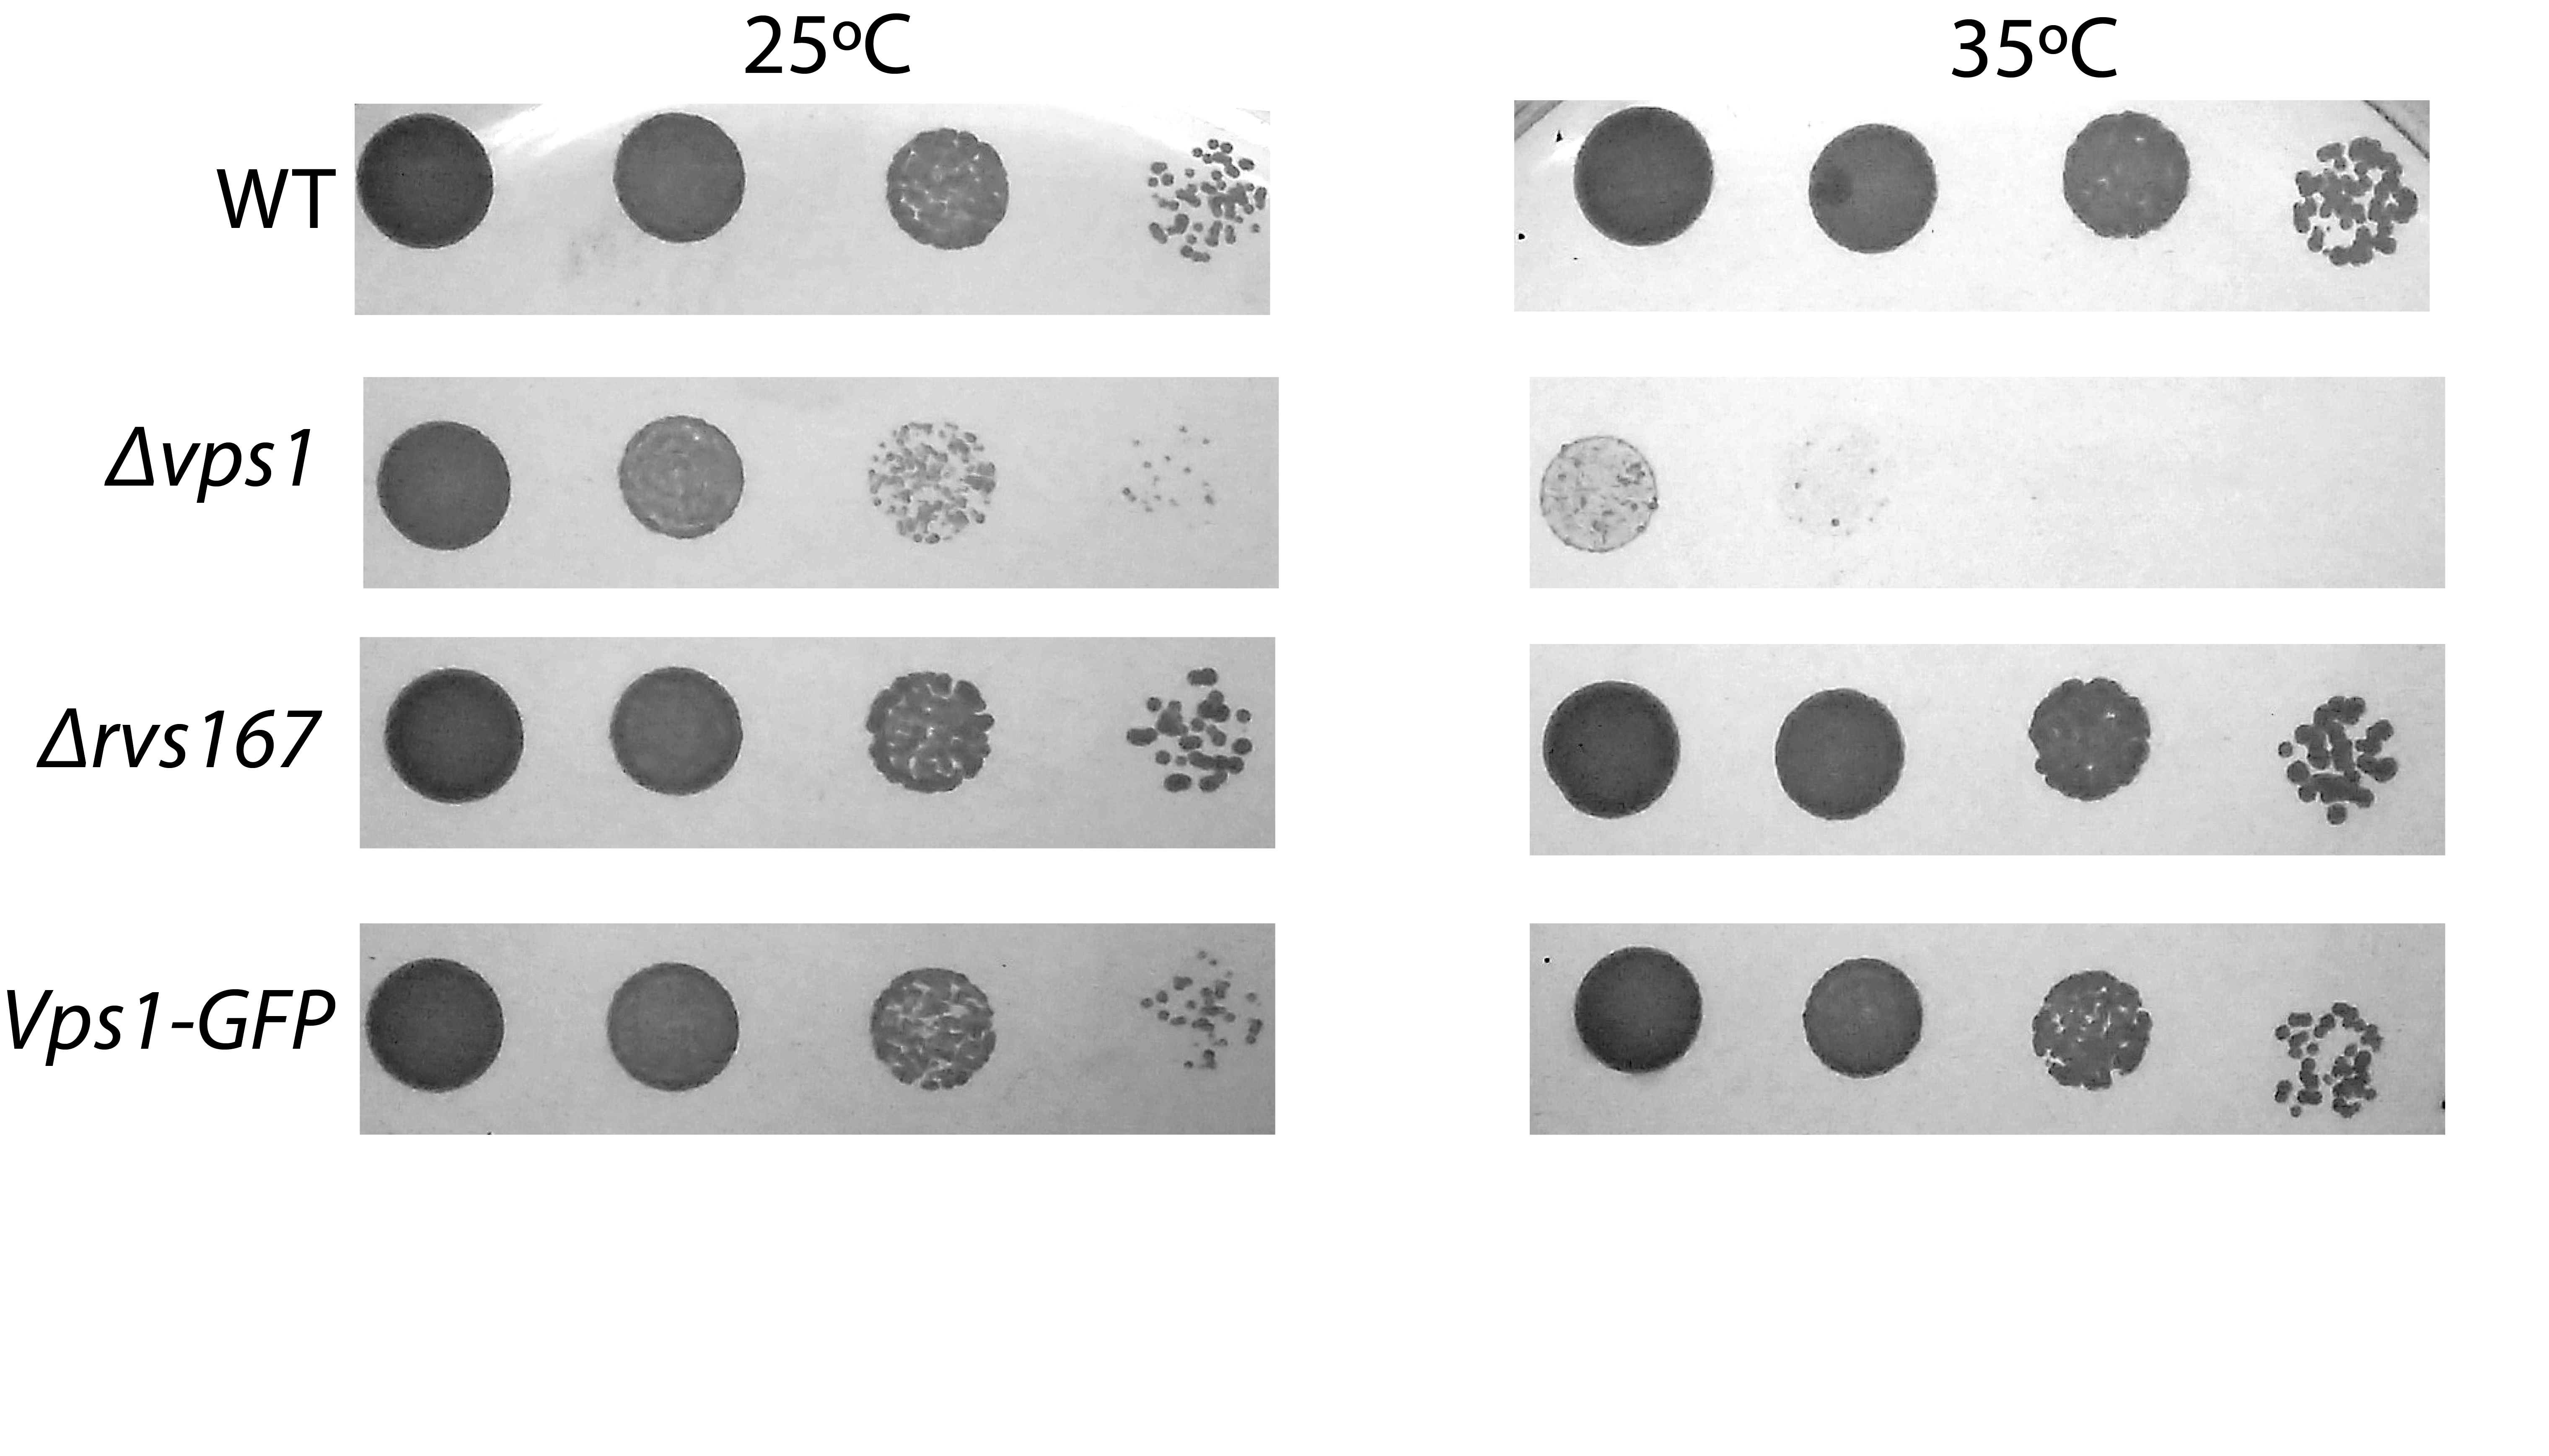
\includegraphics
	[width=0.7\hsize]{/Users/deepikaa/Desktop/scission_paper/figures/fig1/growth_assay.pdf}
	\caption{\textbf { 	Growth assay of WT,  \textit{vps1$\Delta$}, \textit{rvs167$\Delta$}, and cells expressing Vps1-eGFP at 25\si{\degree}C and 35\si{\degree}C } }
	\label{vps_growthassay}
\end{figure}

\begin{figure}[h]
	\centering
	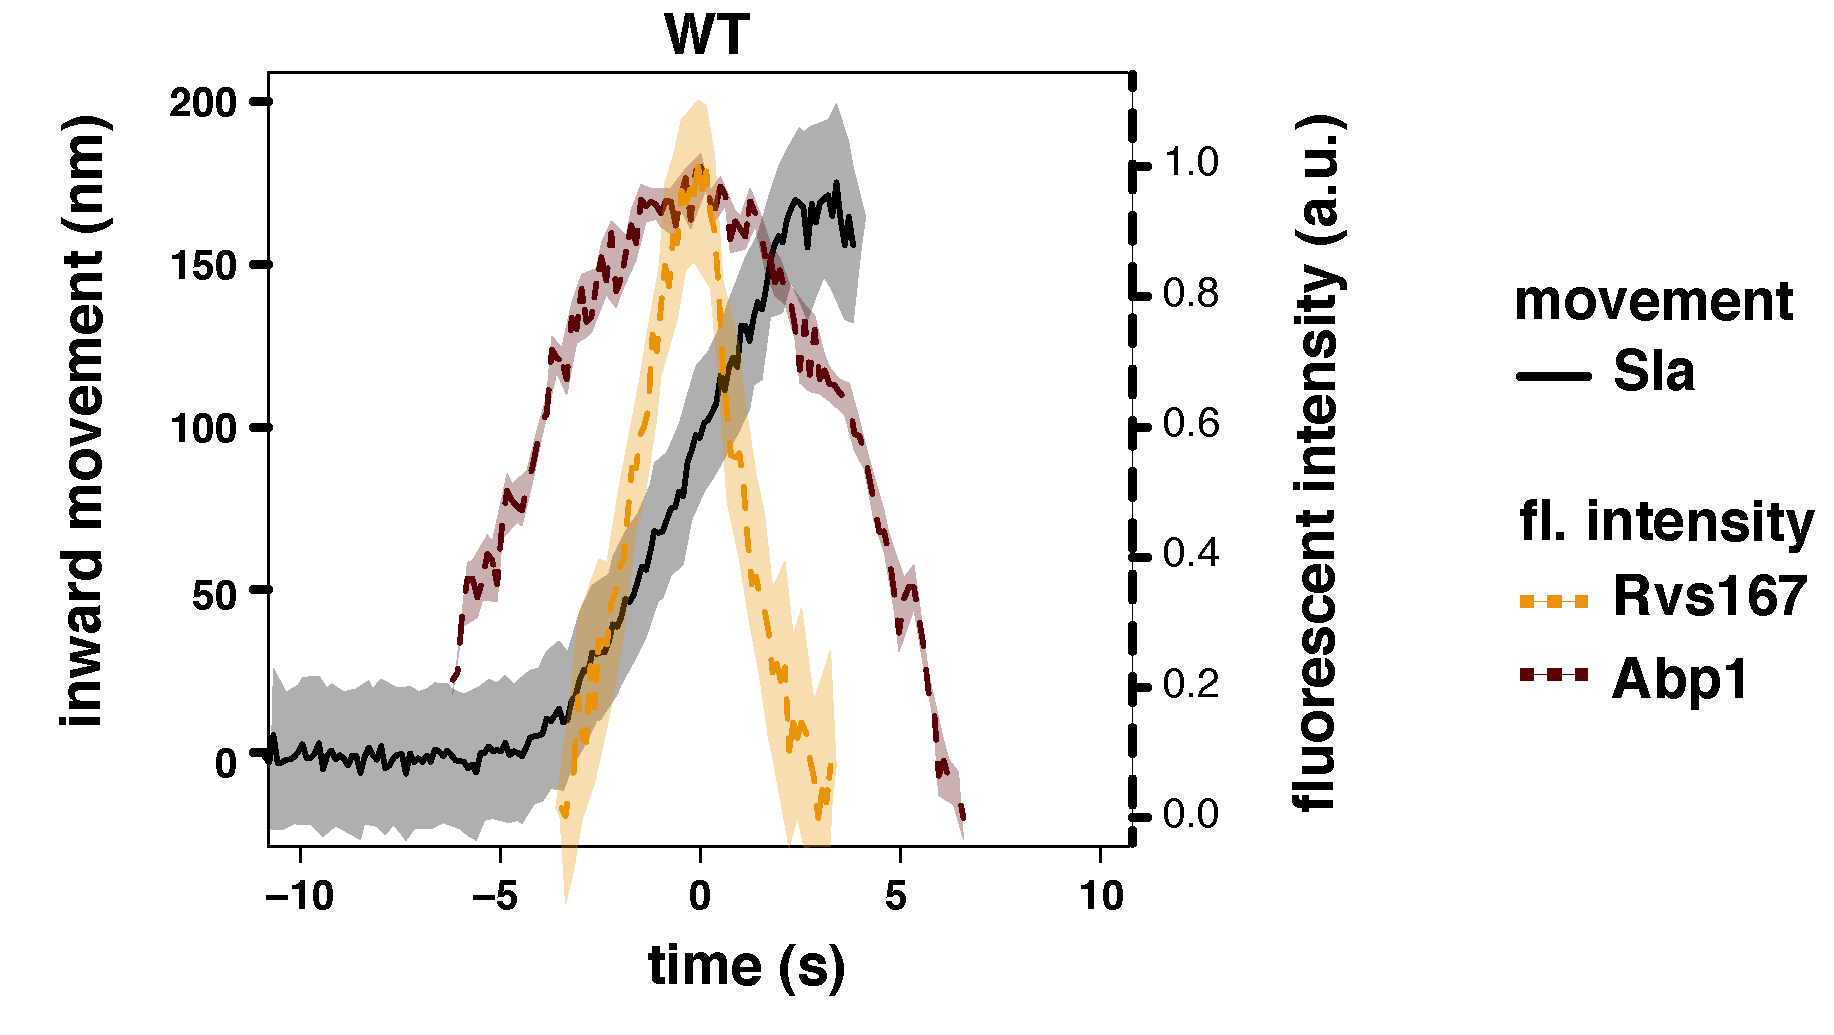
\includegraphics
	[width=0.8\hsize]{/Users/deepikaa/Desktop/scission_paper/figures/fig1/wt_alignment2.pdf}
	\caption{\textbf { Sla1 centroid aligned so that time=0(s) is the maximum of Abp1 fluorescent intensity in \textit{vps1$\Delta$} cells (\cite{Picco2015}), normalized Abp1 and Rvs167 fluorescent  intensities in \textit{vps1$\Delta$} cells }}
	\label{wt_alignment}
\end{figure}

\begin{figure}[h]
	\centering
	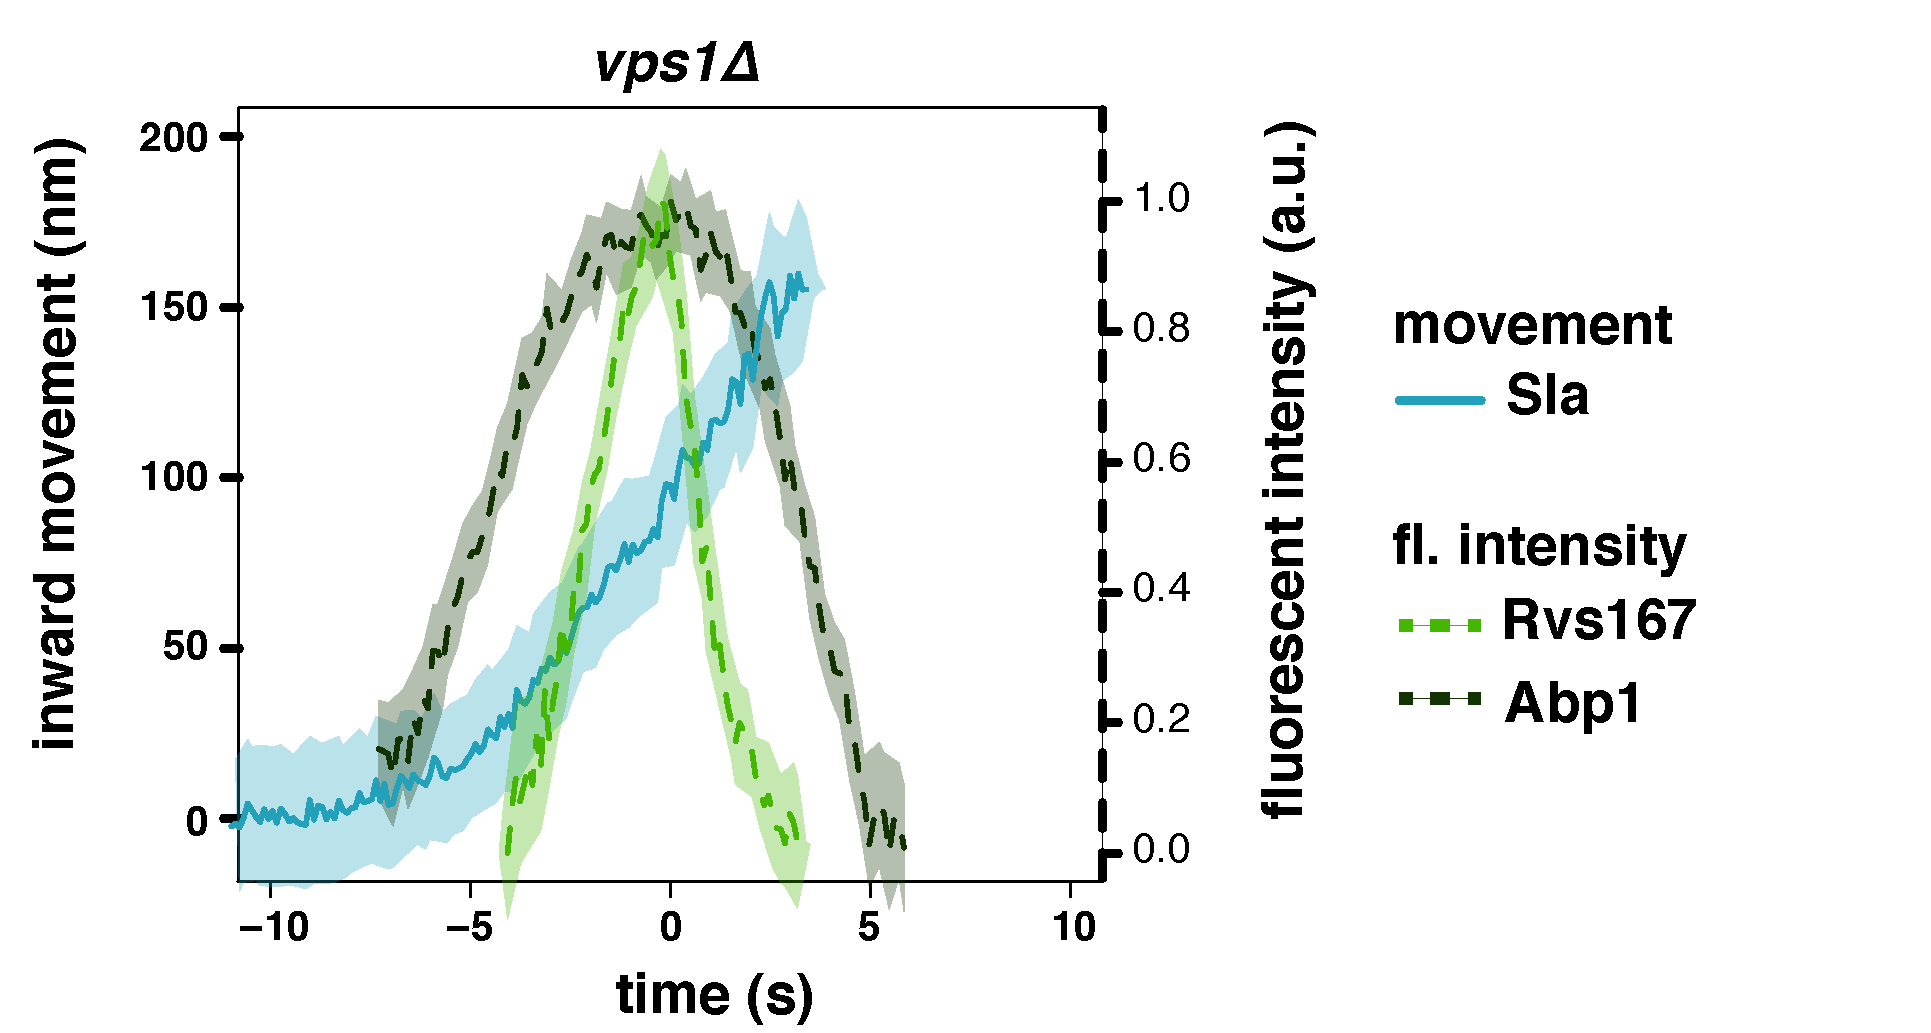
\includegraphics
	[width=0.85\hsize]{/Users/deepikaa/Desktop/scission_paper/figures/fig1/vpsdel_alignment2.pdf}
	\caption{\textbf {  Sla1 centroid aligned so that time=0(s) is the maximum of Abp1 fluorescent intensity in \textit{vps1$\Delta$} cells (\cite{Picco2015}), normalized Abp1 and Rvs167 fluorescent  intensities in \textit{vps1$\Delta$} cells  } }
	\label{vpsdel_alignment}
\end{figure}

\begin{figure}
	\centering
	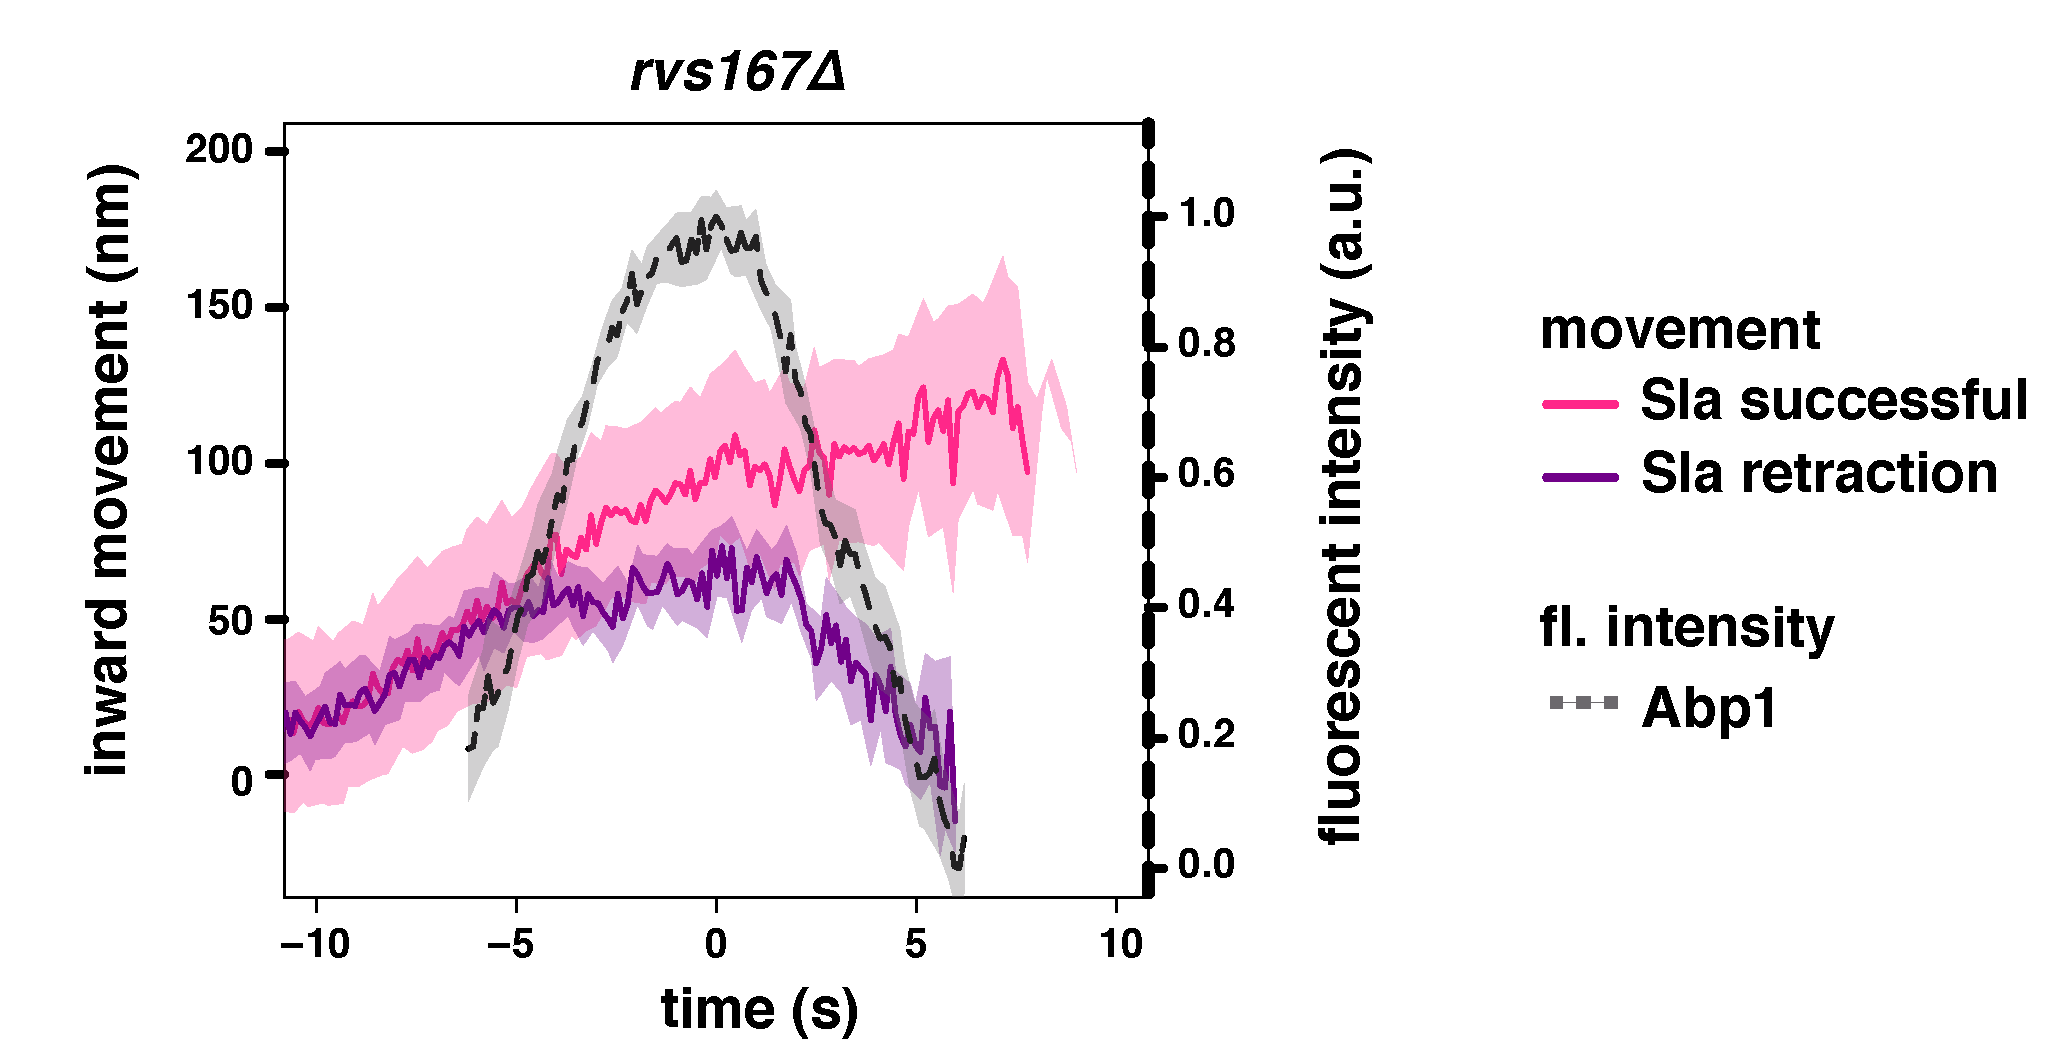
\includegraphics
	[width=0.8\hsize]{/Users/deepikaa/Desktop/scission_paper/figures/fig1/rvsdel_alignment.pdf}
	\caption{\textbf {Sla1 centroid aligned so that time=0(s) is the maximum of Abp1 fluorescent intensity in \textit{rvs167$\Delta$} cells (\cite{Picco2015}), normalized Abp1 fluorescent  intensity in \textit{rvs167$\Delta$} cells }}
	\label{rvsdel_alignment}
\end{figure}

\begin{figure}
	\centering
	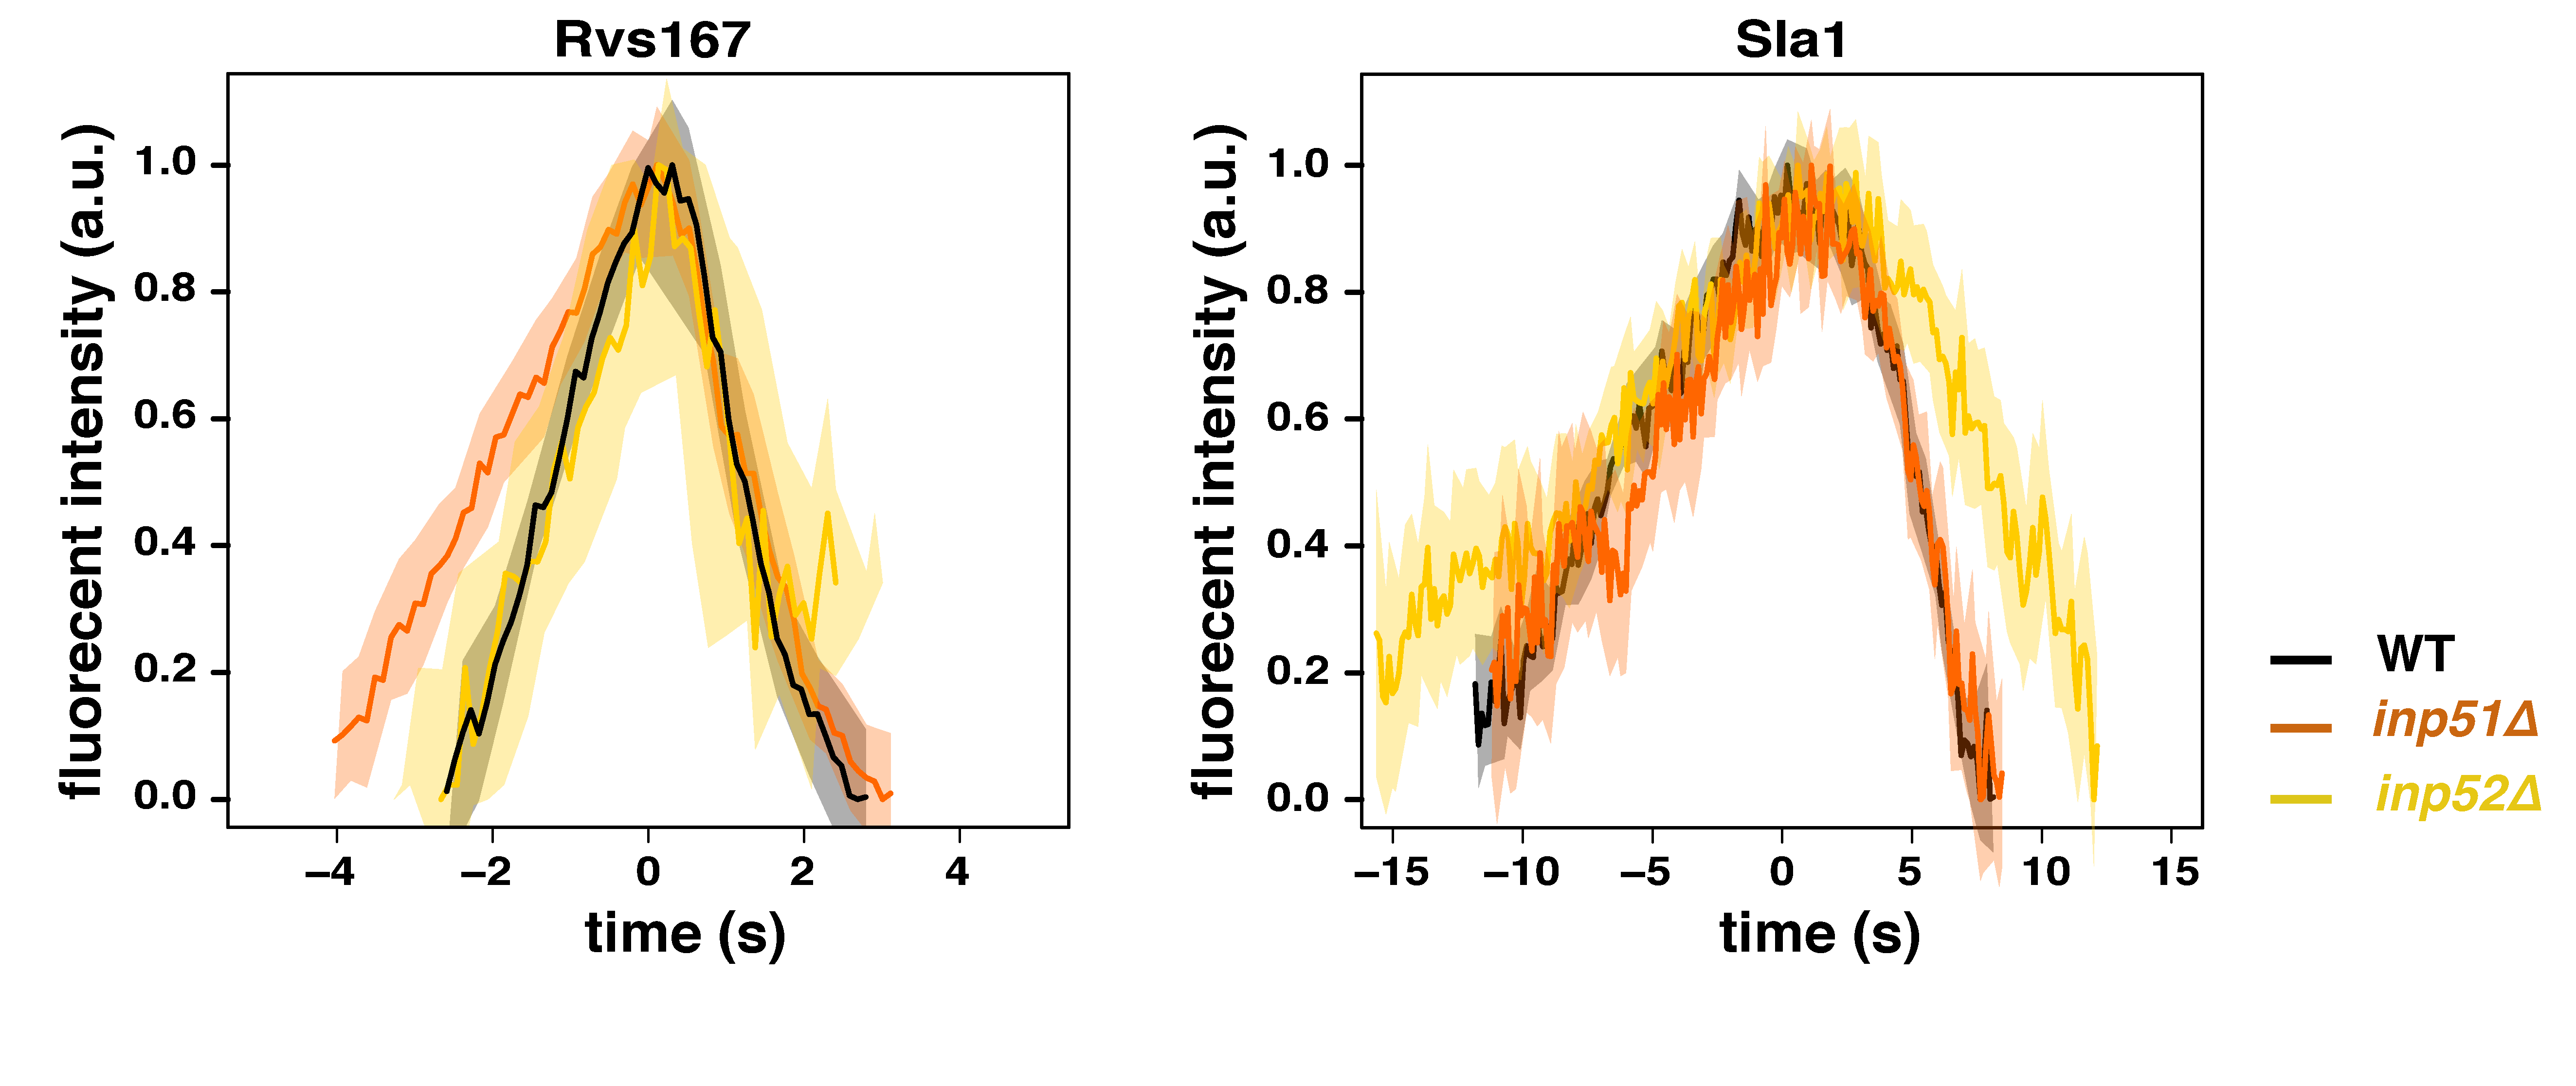
\includegraphics
	[width=0.95\hsize]{/Users/deepikaa/Desktop/scission_paper/figures/fig2/supplement.pdf}
	\caption{\textbf {Sla1 centroid aligned so that time=0(s) is the maximum of Abp1 fluroescent intensity in WT cells (\cite{Picco2015}), normalized Abp1 and Rvs167 fluorescent  intensities in WT cells }}
	\label{inpdel_supplement}
\end{figure}

\begin{figure}
	\centering
	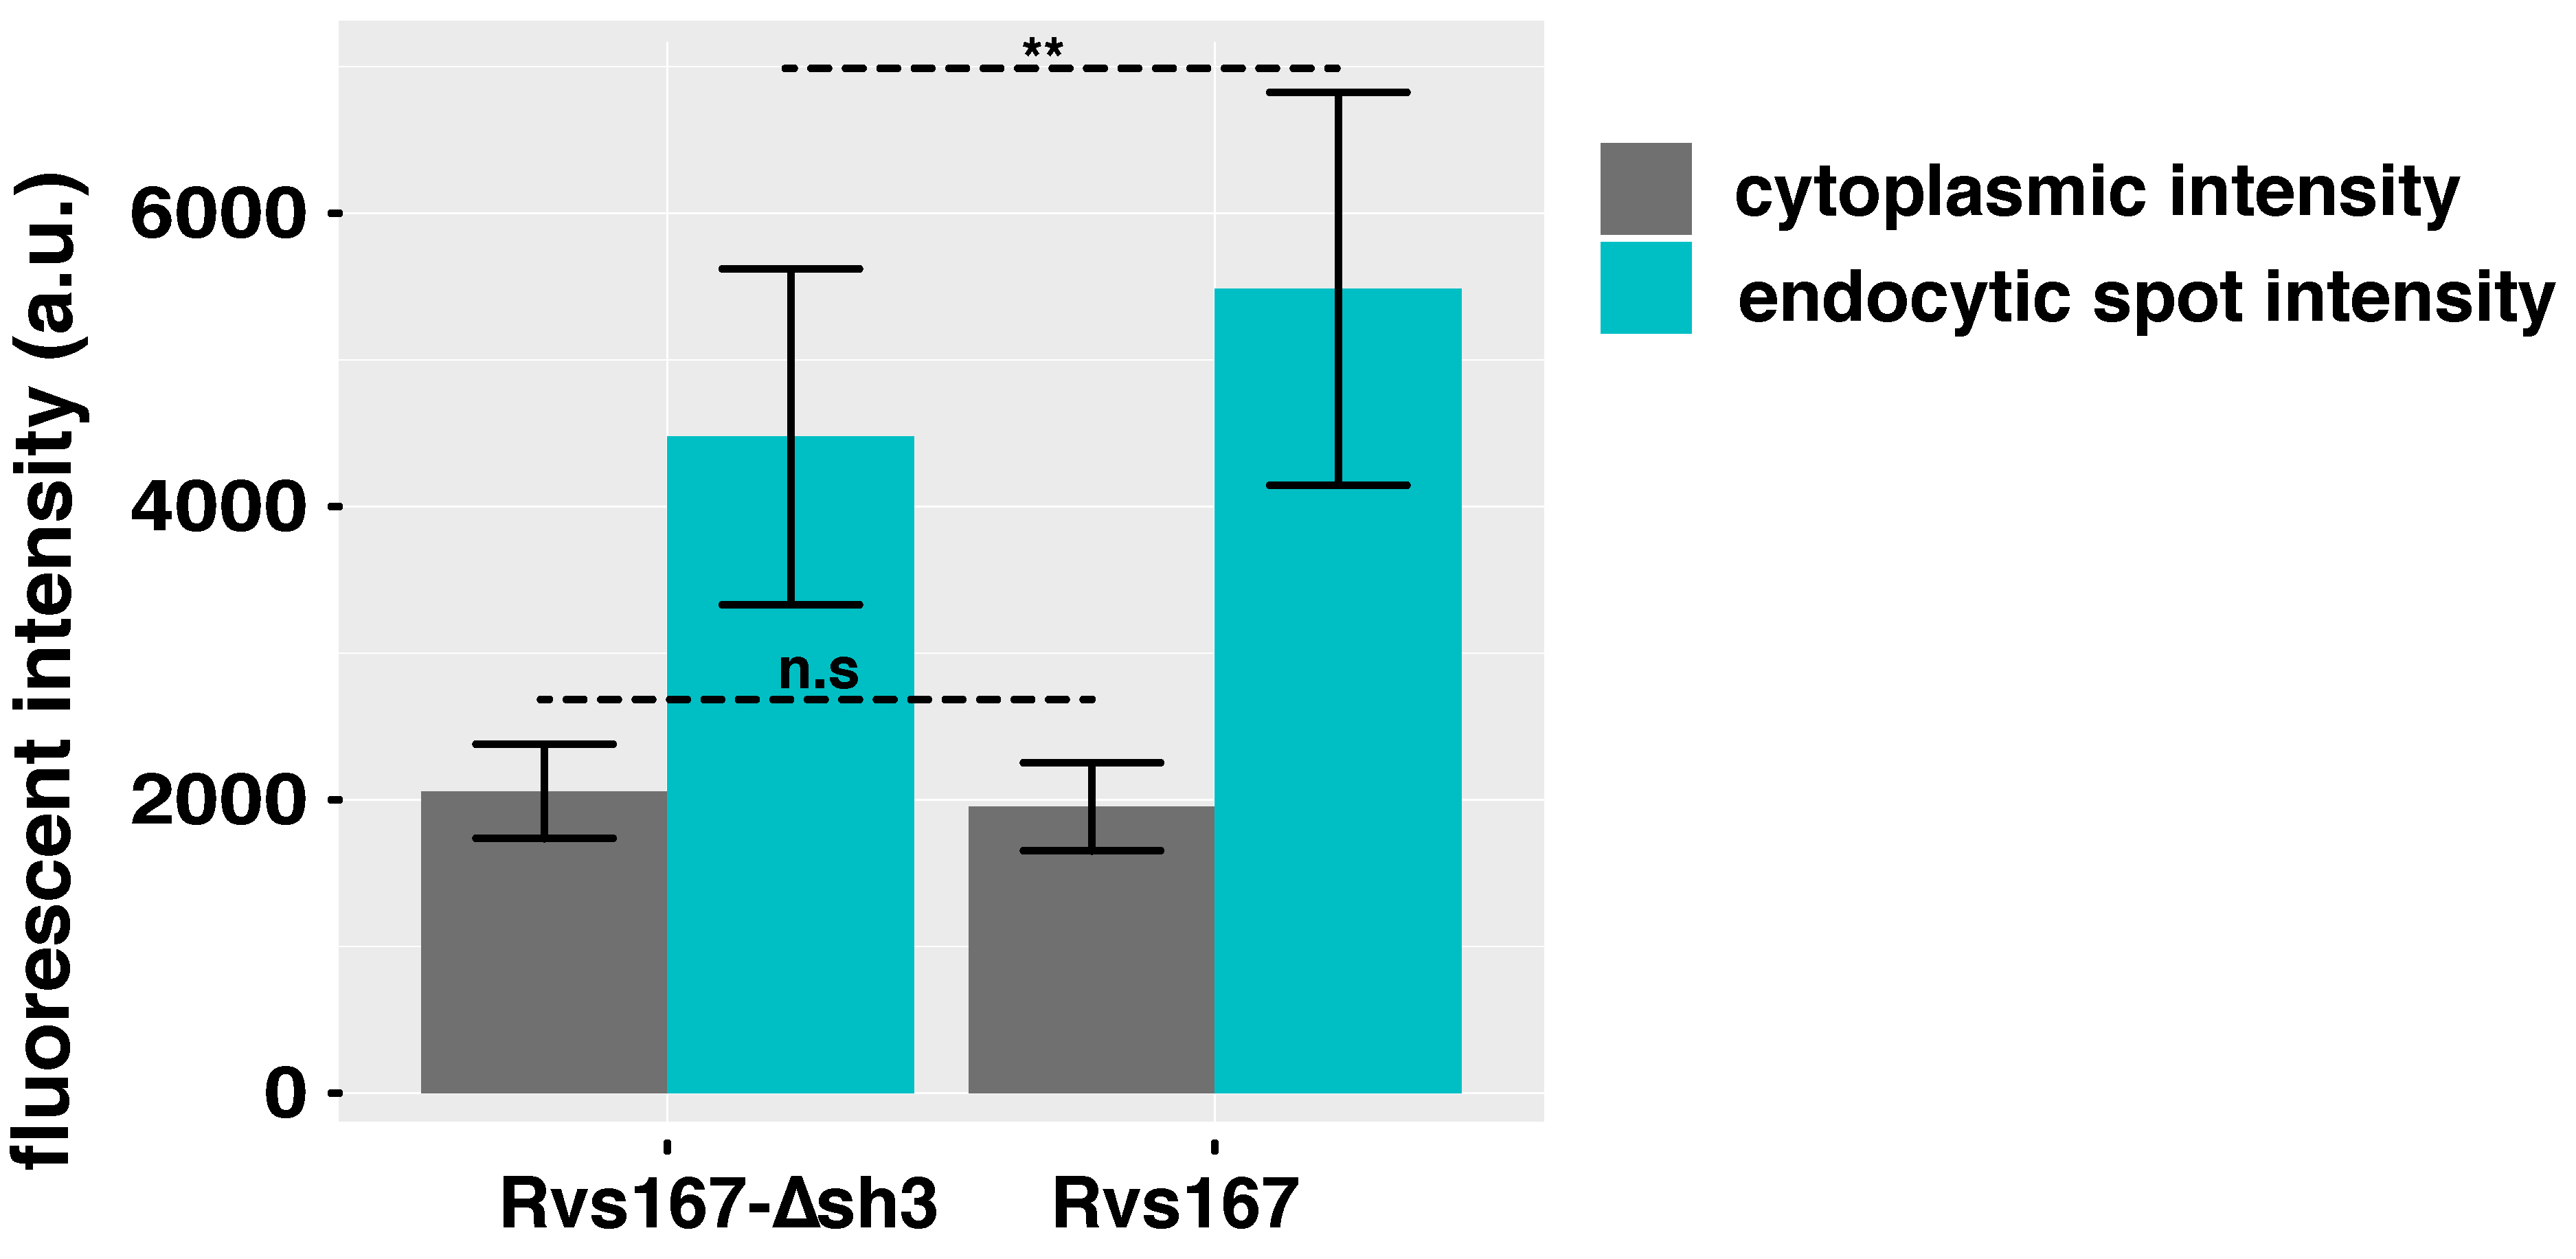
\includegraphics
	[width=0.6\hsize]{/Users/deepikaa/Desktop/scission_paper/figures/fig4/cytoplasmic_int_supplement3.pdf}
	\caption{\textbf { Cytoplasmic intensity and intensity of endocytic patches of Rvs167 and Rvs167\textit{$\Delta$sh3} in WT and \textit{rvs167$\Delta$sh3} cells}}
	\label{delsh3_cytoplasmic}
\end{figure}

\end{document}
